\chapter{Analysis of SMELLIE Data in the Scintillator Phase}\label{chap:smellie_analysis}
% \epigraph{\textit{}}{source}

This chapter contains two sets of analyses: measurements of the extinction lengths of the scintillator as a function of wavelength and time, as well as monitoring the Rayleigh scattering length over time. In both cases, care had to be taken to try and make the methodologies robust to systematics.

\section{Extinction Length Analysis}\label{sec:ext_length_analysis}
% \subsection{Motivation}
% \begin{itemize}
%     \item Explain motivating observations for this analysis: a substantial discrepancy between MC and data seen in the radial profiles of nhitsCleaned for \ce{^{210}Po} after the PPO top-up campaign. Performed by Serena.
%     \item Hypothesis of a shortening of the absorption/scattering length proposed, further strengthened by Ben Tam's ex-situ absorption measurements with scintillator taken from the detector, as well as knowledge about a likely ``cooking'' of PPO during the PPO-fill.
%     \item Describe the provisional optics model decided on based on these measurements, which includes an additional non-re-emitting component of the scintillator.
%     \item As a further cross-check, SMELLIE should be sensitive to changes in the overall extinction length of the scintillator, especially for short extinction lengths relative to the size of the detector.
%     \item More straightforward in measuring extinction length compared to scattering length --- no need to distinguish between scintillator re-emission and scattering.
%     \item Further uses: can be used to monitor the extinction length over time!
% \end{itemize}
% [4 pages]
The first analysis discussed in this chapter is the measurement of the extinction lengths of the liquid scintillator deployed in the SNO+ detector, as a function of both wavelength and time. As seen in Fig.~\ref{fig:smellie_timeline}, SMELLIE data was taken during the water phase, and in the scintillator phase when the PPO concentration of the LABPPO was at a variety of levels. Fig.~\ref{fig:smellie_expected_ext_length_phases} shows the expected changes in extinction length with detector phase, as a function of wavelength, according to the optical model described in Section~\ref{sec:optical_processes}.

\begin{figure}
    \centering
    % 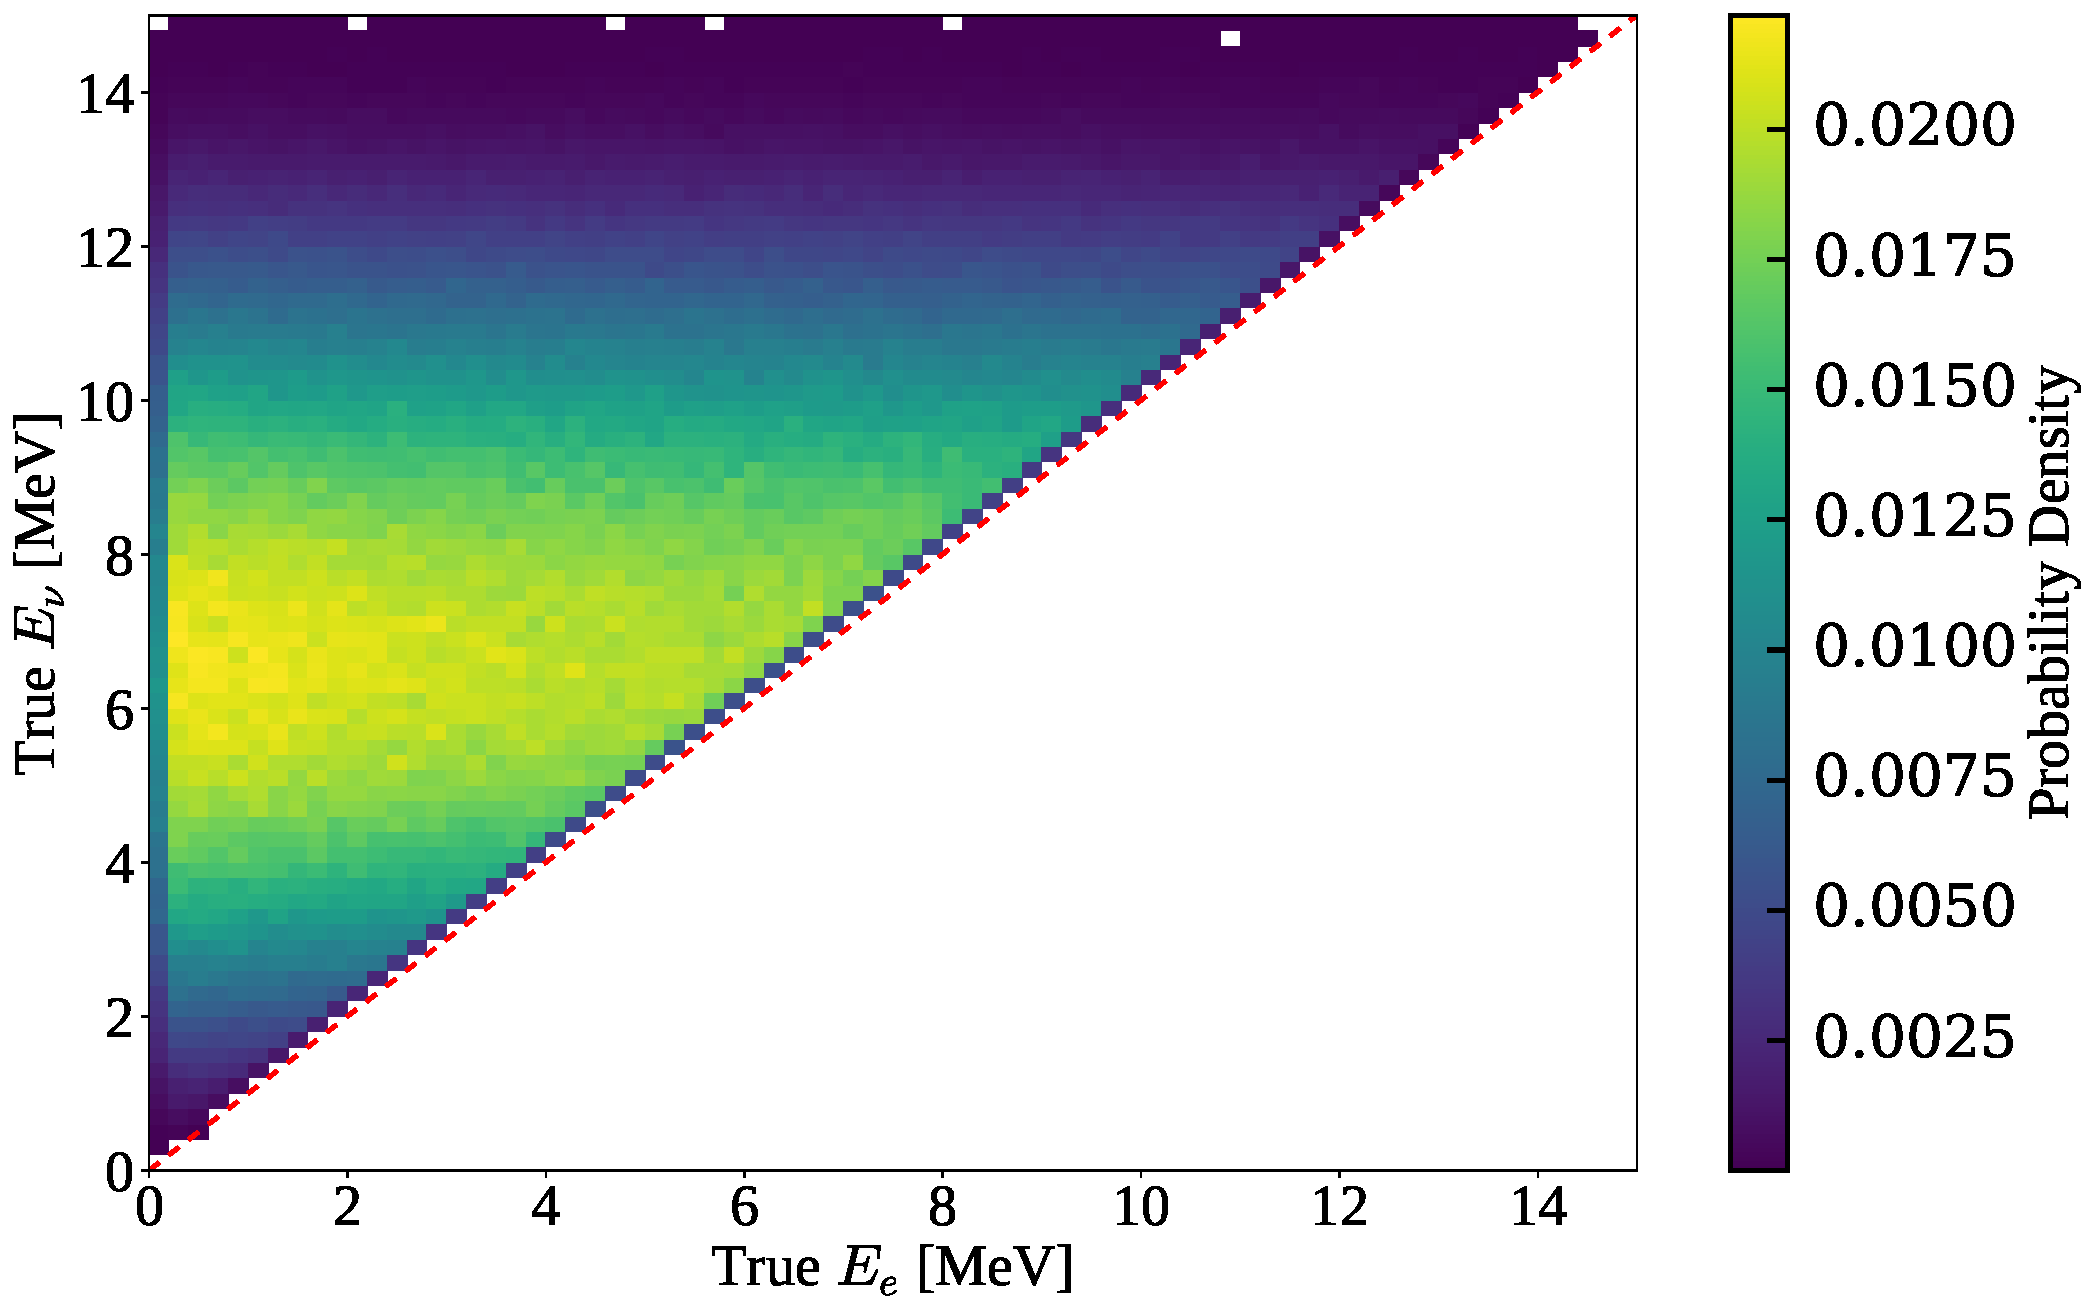
\includegraphics[width=0.8\textwidth]{6_SolarAnalysis/images/b8_eelectrue_vs_enutrue.pdf}
    \caption[]{}
    \label{fig:smellie_expected_ext_length_phases}
\end{figure}

\subsection{Mathematical Model}
To begin, consider light emission from a particular SMELLIE fibre of fixed wavelength $\lambda_{j}$, with a mean emission intensity of $I_{j}$ photons emitted per event in subrun $j$ during detector phase $p$. Modifying Eq.~\ref{eq:mu_def}, a general PMT $i$ will have a mean npe per event of $\mu_{ij,p}(\lambda_{j}) = I_{j,p}b_{i,p}(\lambda_{j})f_{i,p}(\lambda_{j})$. A detector phase-dependence has been added to all terms, because:
\begin{itemize}
    \item The emission intensities chosen, $I_{j,p}$, can vary between different data-taking campaigns. These changes are due to changes in hardware (as detailed in Chapter~\ref{chap:smellie_hardware}), as well as changes in the settings used to run SMELLIE.
    \item The beam profile of a given fibre at a given wavelength is not expected to change with detector phase. However, if the refractive index of the inner detector medium changes (e.g. from the water phase to scintillator phase), then the fraction of light emitted that is pointed in the correct direction to be detected by PMT $i$, $b_{i,p}(\lambda_{j})$, \textit{can} change.
    \item In a different phase of the detector, the optics of the inner detector can change. As a result, the probability that a photon pointing in the correct direction for PMT $i$ actually makes it across the detector and generates a photoelectron, $f_{i,p}(\lambda_{j})$, can change.
\end{itemize}

\begin{figure}
    \centering
    % 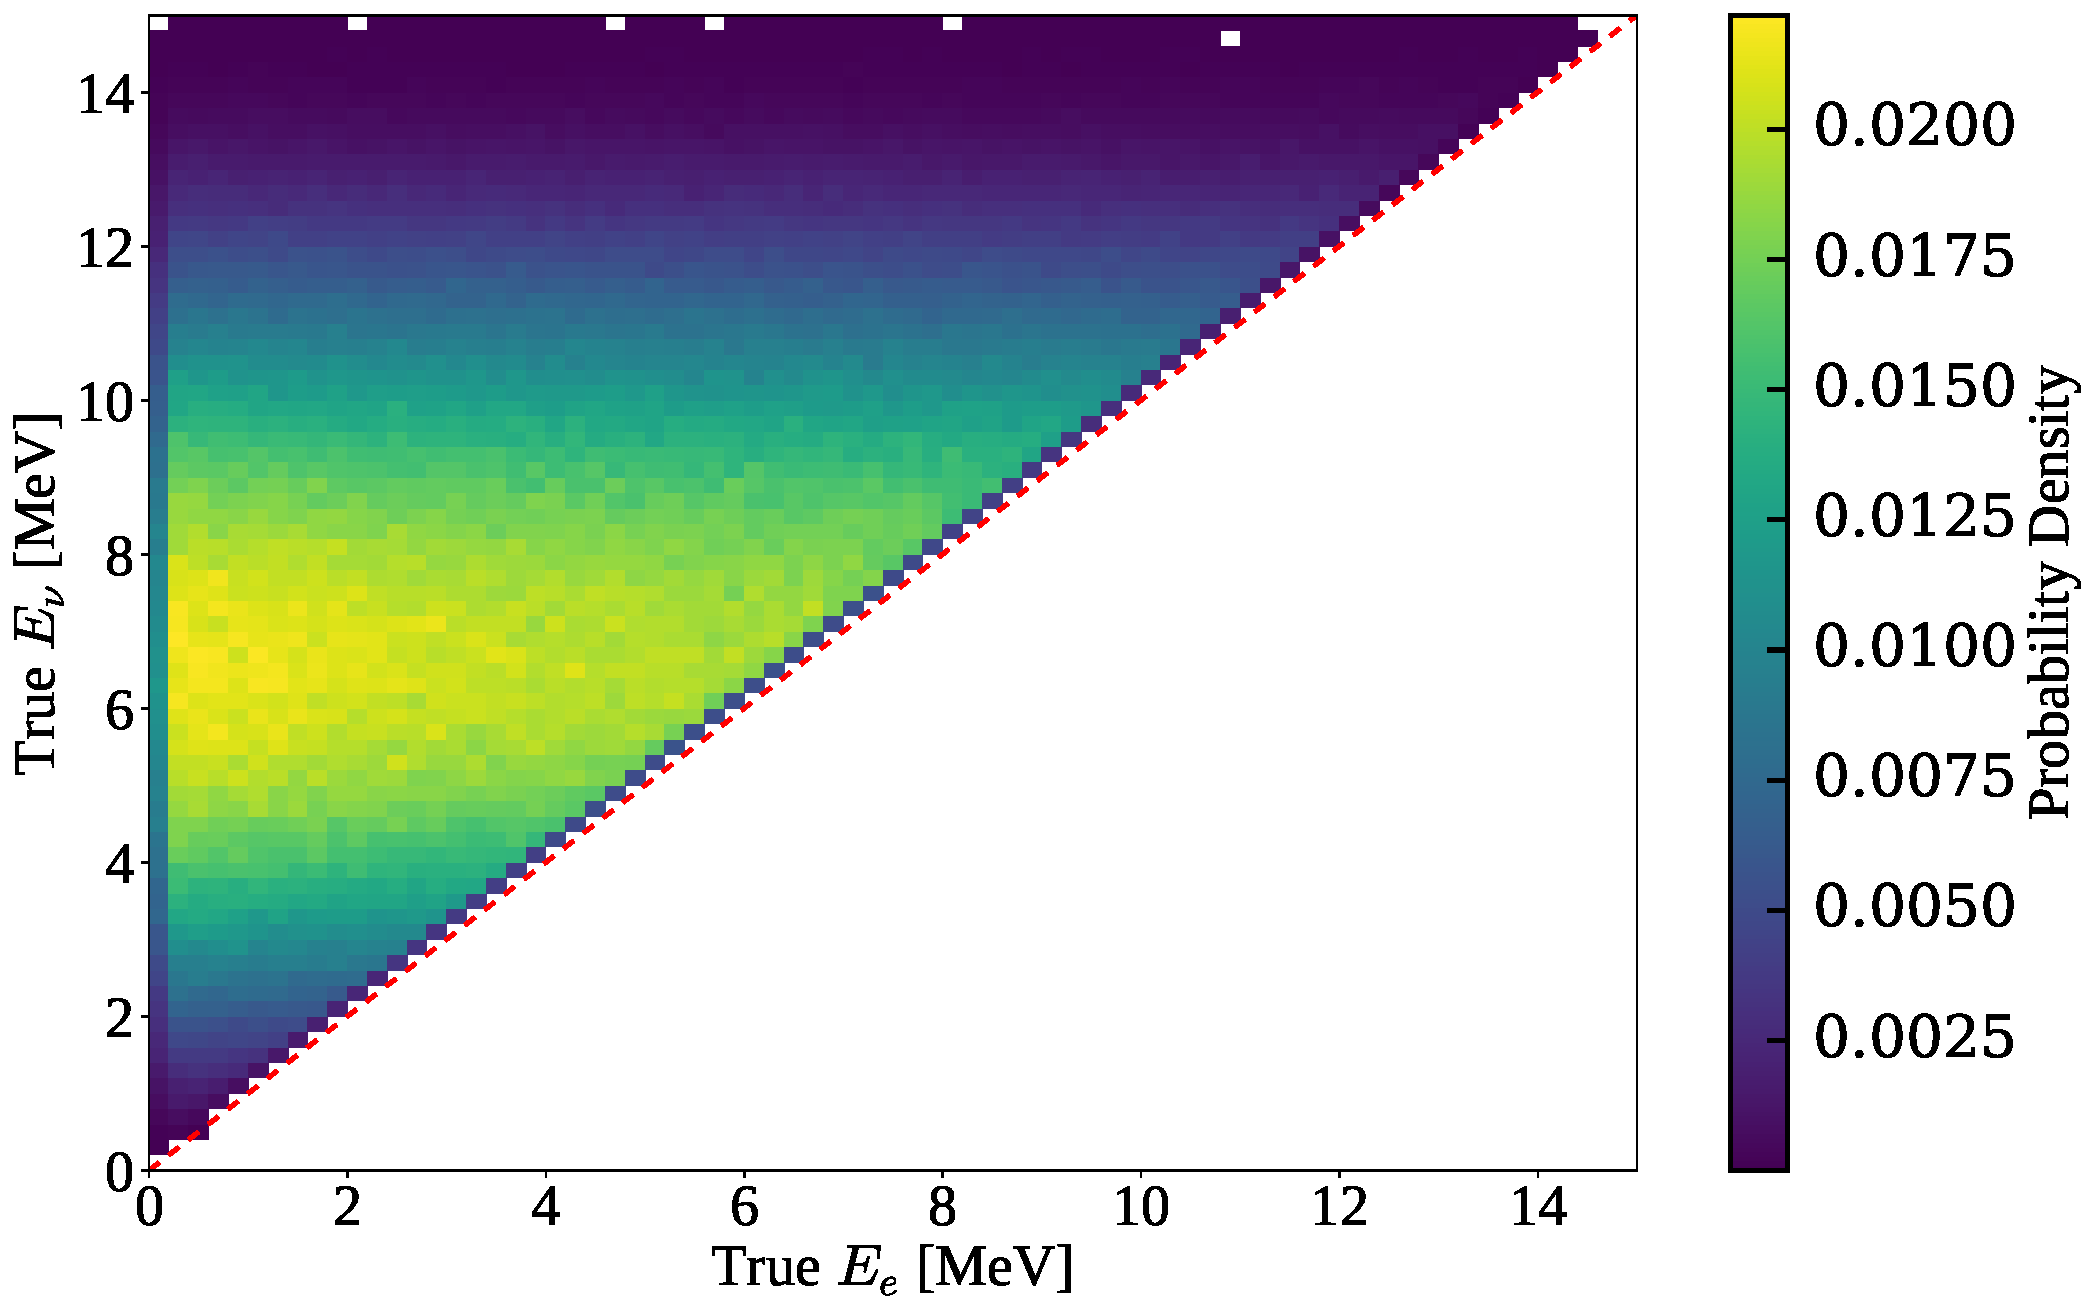
\includegraphics[width=0.8\textwidth]{6_SolarAnalysis/images/b8_eelectrue_vs_enutrue.pdf}
    \caption[]{}
    \label{fig:smellie_ext_length_schematic}
\end{figure}

In this analysis, two regions of PMTs will be used for a given fibre; Fig.~\ref{fig:smellie_ext_length_schematic} shows a schematic of the PMT selections. The first region corresponds to PMTs \textit{radially-opposite} the fibre emission point in the detector, i.e. the lightpaths travel orthogonally through all surface boundaries. The reason for this choice will be explained shortly. Considering the various contributions to the value of $f_{i,p}(\lambda_{j})$, a PMT in this `far' selection will have a mean npe per event, $\mu_{ij,p}^{\mathrm{far}}(\lambda_{j})$, of:
\begin{align}\label{eq:smellie_ext_length_theory}
    \mu_{ij,p}^{\mathrm{beam}}(\lambda_{j}) &= I_{j,p}b_{i,p}(\lambda_{j})
    \exp\left(
        -\frac{L_{ij,p}^{\mathrm{extern}}(\lambda_{j})}{l^{\mathrm{extern}}(\lambda_{j})}
    \right)
    \exp\left(
        -\frac{L_{ij,p}^{\mathrm{acr}}(\lambda_{j})}{l^{\mathrm{acr}}(\lambda_{j})}
    \right)
    \exp\left(
        -\frac{L_{ij,p}^{\mathrm{inner}}(\lambda_{j})}{l_{p}^{\mathrm{inner}}(\lambda_{j})}
    \right)\nonumber\\
    & \qquad\cdot T_{ij,p}(\lambda_{j})\epsilon_{ij,p}(\lambda_{j}).
\end{align}
Here, $L_{ij,p}^{\mathrm{extern,acr,inner}}(\lambda_{j})$ is the length of a path in a given detector medium through which light travels, for the external water, acrylic, and inner detector medium, respectively. $l_{p}^{\mathrm{extern,acr,inner}}(\lambda_{j})$ is the extinction length of each detector medium for a given wavelength --- it is assumed that only the inner detector medium has changing optics in different phases. Some fraction of light is lost when passing between two mediums with different refractive indices: this is captured by $T_{ij,p}(\lambda_{j})$, the product of the Fresnel transmission components for all optical boundaries along a photon's path. Finally, $\epsilon_{ij,p}(\lambda_{j})$ is the probability that a photon along a given path, incident on a given PMT, will generate a photoelectron that is detected. 

The second selection of PMTs are those near the fibre emission point. The first light observed by these PMTs will be from photons which have `back-scattered' off of the UPW outside the AV. This is followed by light reflected off of the AV surface. Fig.~\ref{fig:smellie_back_PMTs_tres_plot} shows the observed time residual distribution for such a PMT. As can be seen, the back-scattered light is well-separated in time from all other optical processes. % note about rope reflections!
Assuming that the Rayleigh scattering properties of the UPW outside the AV have been unchanged throughout the lifetime of the detector, then the expected number of photoelectrons observed in a selection of these PMTs during a time period in which only back-scattering can occur will be simply:
\begin{equation}
    \mu_{j,p}^{\mathrm{back}} = kI_{j,p}.
\end{equation}
$k$ here is just some general constant of proportionality. Therefore, observing this back-scattered light can be used as a measure of the relative intensity of the subrun.

\begin{figure}
    \centering
    % 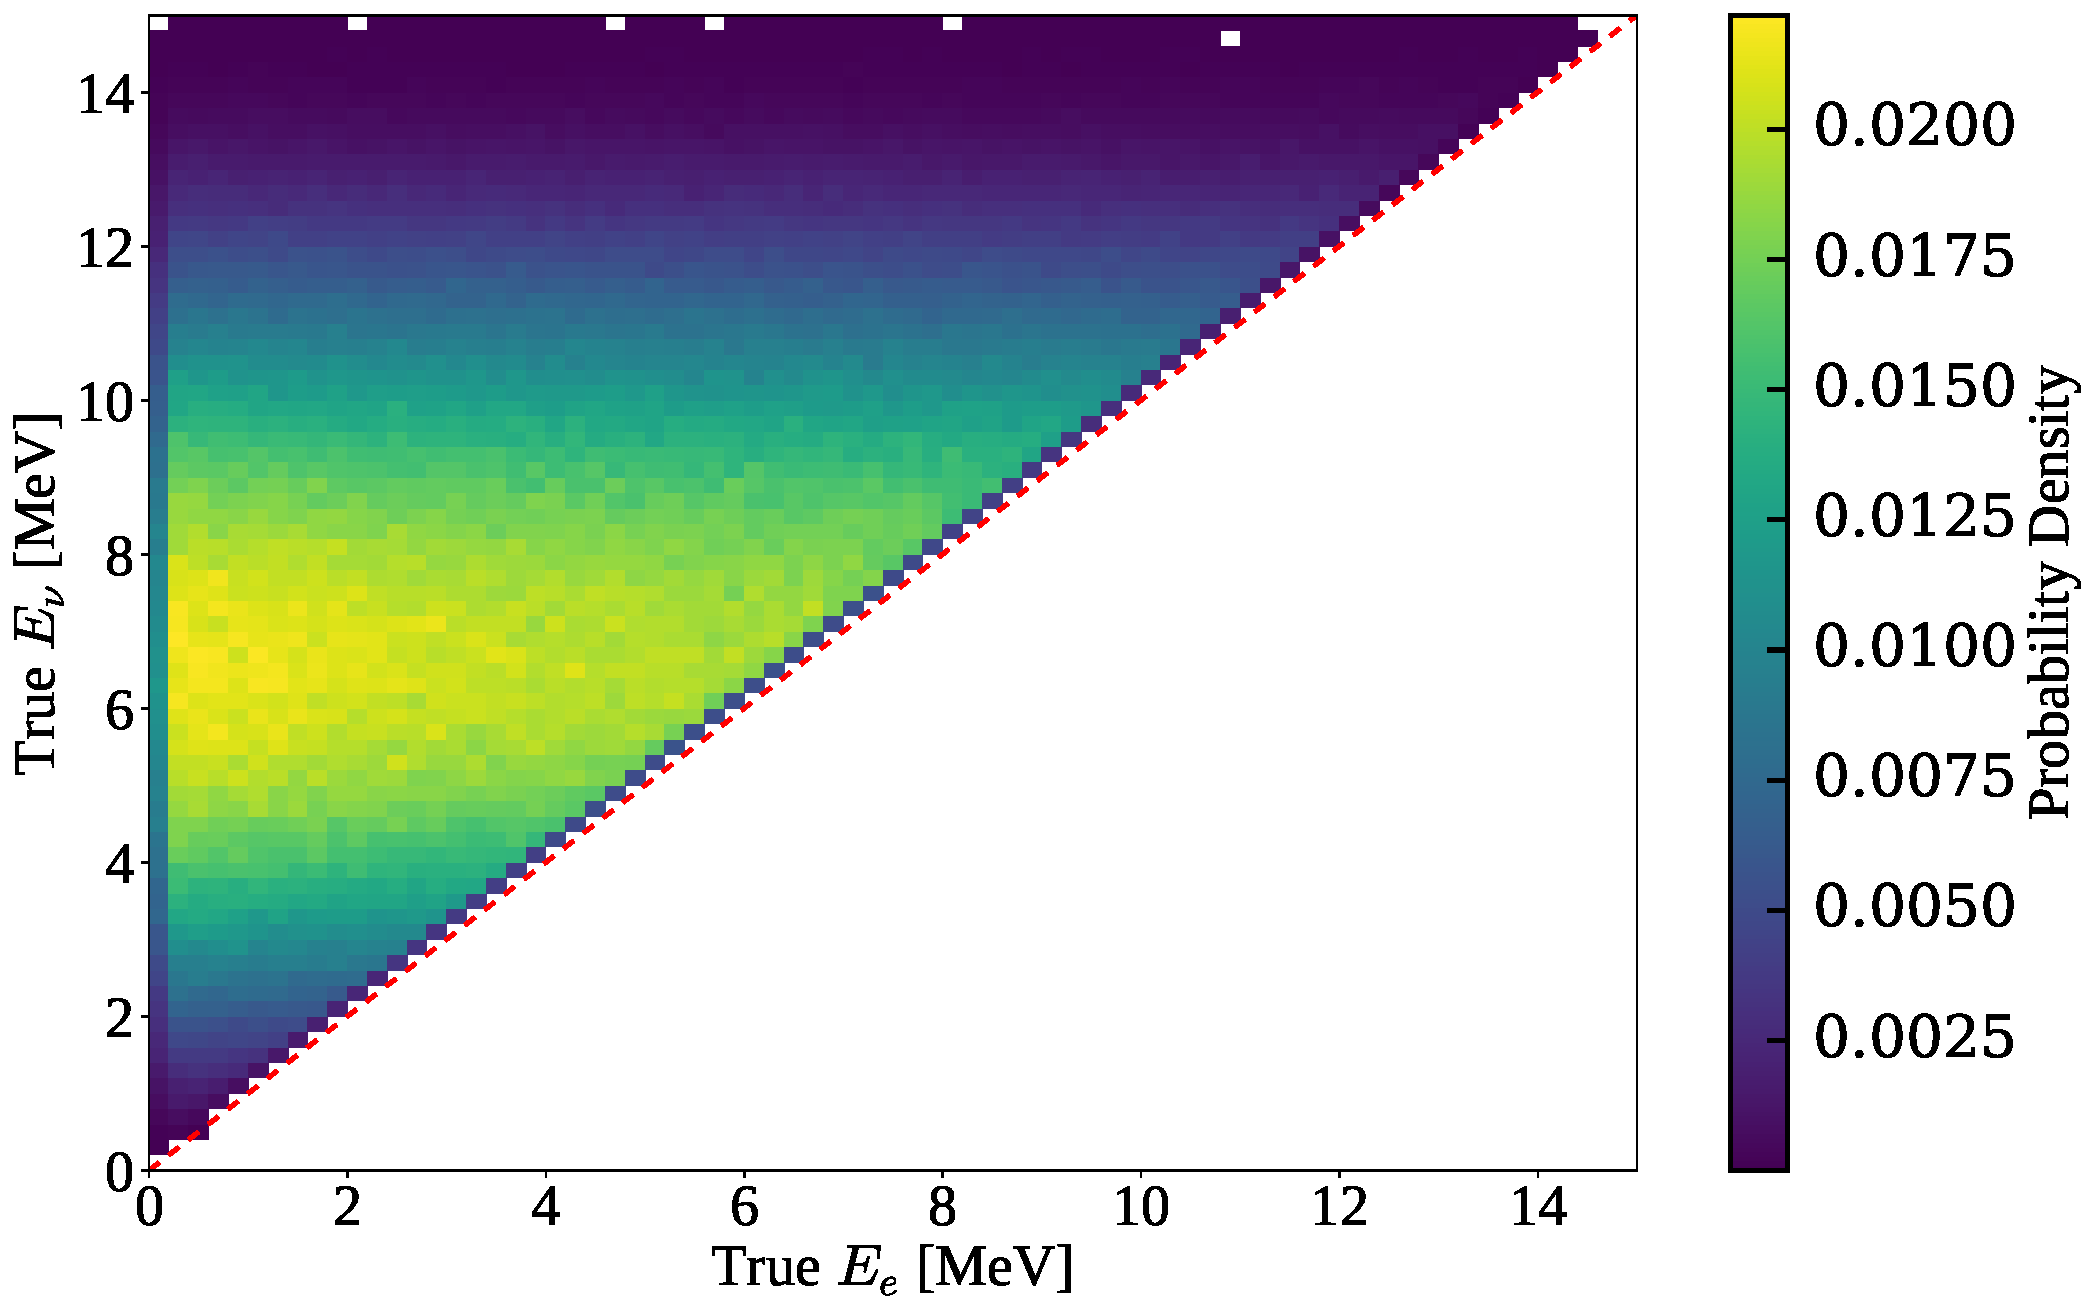
\includegraphics[width=0.8\textwidth]{6_SolarAnalysis/images/b8_eelectrue_vs_enutrue.pdf}
    \caption[]{}
    \label{fig:smellie_back_PMTs_tres_plot}
\end{figure}

Because $\mu_{j,p}^{\mathrm{back}}$ is proportional to the intensity, the ratio $R_{ij,p} = \mu_{ij,p}^{\mathrm{beam}}(\lambda_{j})/\mu_{j,p}^{\mathrm{back}}$ will be independent of $I_{j,p}$. A similar trick can be used to remove the dependence of $R_{ij,p}$ on $k$, by taking the ratio of $R_{ij,p}$ with $R_{ij,\ce{H_{2}O}}$, where $R_{ij,\ce{H_{2}O}}$ is the measured values of $R_{ij,p}$ in the water phase. This ratio becomes:
\begin{align}
    \frac{R_{ij,p}}{R_{ij,\ce{H_{2}O}}}(\lambda_{j}) 
    &= \frac{k}{k}
    \frac{b_{i,p}(\lambda_{j})}{b_{i,\ce{H_{2}O}}(\lambda_{j})}
    \frac{T_{ij,p}(\lambda_{j})}{T_{ij,\ce{H_{2}O}}(\lambda_{j})}
    \frac{\epsilon_{ij,p}(\lambda_{j})}{\epsilon_{ij,\ce{H_{2}O}}(\lambda_{j})}
    \exp\left(
        -\frac{L_{ij,p}^{\mathrm{extern}}(\lambda_{j})-L_{ij,\ce{H_{2}O}}^{\mathrm{extern}}(\lambda_{j})}{l^{\mathrm{extern}}(\lambda_{j})}
    \right)
    \nonumber\\
    & \quad \cdot \exp\left(
        -\frac{L_{ij,p}^{\mathrm{acr}}(\lambda_{j})-L_{ij,\ce{H_{2}O}}^{\mathrm{acr}}(\lambda_{j})}{l^{\mathrm{acr}}(\lambda_{j})}
    \right)
    \exp\left(
        -\frac{L_{ij,p}^{\mathrm{inner}}(\lambda_{j})}{l_{p}^{\mathrm{inner}}(\lambda_{j})}
        +\frac{L_{ij,\ce{H_{2}O}}^{\mathrm{inner}}(\lambda_{j})}{l_{\ce{H_{2}O}}^{\mathrm{inner}}(\lambda_{j})}
    \right)
    \nonumber\\
    &= \frac{b_{i,p}(\lambda_{j})\epsilon_{ij,p}(\lambda_{j})}{b_{i,\ce{H_{2}O}}(\lambda_{j})\epsilon_{ij,\ce{H_{2}O}}(\lambda_{j})}
    \frac{T_{ij,p}(\lambda_{j})}{T_{ij,\ce{H_{2}O}}(\lambda_{j})}
    \exp\left(
        -\frac{L_{ij,p}^{\mathrm{inner}}(\lambda_{j})}{l_{p}^{\mathrm{inner}}(\lambda_{j})}
        +\frac{L_{ij,\ce{H_{2}O}}^{\mathrm{inner}}(\lambda_{j})}{l_{\ce{H_{2}O}}^{\mathrm{inner}}(\lambda_{j})}
    \right),
\end{align}
where it has been assumed that any change in path length through the external UPW or acrylic relative to their extinction lengths is negligible.

Importantly, when considering the first PMT selection, a further simplification can be made to the above formula. Because the light travels orthogonally through the AV boundaries, its path is unaffected by changes in the refractive index of the inner detector medium. Therefore, the impact of the beam profile and PMT efficiency will be unchanged, and so the formula simplifies to:
\begin{equation}\label{eq:smellie_ext_length_rsrw_formula_1PMT}
    R_{ij,p}(\lambda_{j}) = 
    \frac{T_{ij,p}(\lambda_{j})}{T_{ij,\ce{H_{2}O}}(\lambda_{j})}
    \exp\left(
        -\frac{L_{ij,p}^{\mathrm{inner}}(\lambda_{j})}{l_{p}^{\mathrm{inner}}(\lambda_{j})}
        +\frac{L_{ij,\ce{H_{2}O}}^{\mathrm{inner}}(\lambda_{j})}{l_{\ce{H_{2}O}}^{\mathrm{inner}}(\lambda_{j})}
    \right)
    \cdot R_{ij,\ce{H_{2}O}}(\lambda_{j}).
\end{equation}
The measurable quantities $R_{ij,\ce{H_{2}O}}(\lambda_{j})$ and $R_{ij,p}(\lambda_{j})$ are then proportional to one another, with the constant of proportionality being a function of the variable of interest $l_{p}^{\mathrm{inner}}(\lambda_{j})$.

% Rearranging the above for $l_{p}^{\mathrm{inner}}(\lambda_{j})$, one can write:
% \begin{align}\label{eq:smellie_ext_length_1PMT}
%     l_{p}^{\mathrm{inner}}(\lambda_{j}) &= 
%     \frac{
%         L_{ij,p}^{\mathrm{inner}}(\lambda_{j})
%         }{
%         \ln\left(
%             \frac{R_{ij,\ce{H_{2}O}}}{R_{ij,p}}(\lambda_{j})\cdot s_{ij,p}(\lambda_{j})
%         \right)
%         + \ln\left(
%             \frac{T_{ij,p}(\lambda_{j})}{T_{ij,\ce{H_{2}O}}(\lambda_{j})}
%         \right)
%         + \frac{L_{ij,\ce{H_{2}O}}^{\mathrm{inner}}(\lambda_{j})}{l_{\ce{H_{2}O}}^{\mathrm{inner}}(\lambda_{j})}
%     },\nonumber\\
%     s_{ij,p}(\lambda_{j}) &=
%     \frac{
%         b_{i,\ce{H_{2}O}}(\lambda_{j})\epsilon_{ij,\ce{H_{2}O}}(\lambda_{j})
%         }{
%         b_{i,p}(\lambda_{j})\epsilon_{ij,p}(\lambda_{j})
%     }.
% \end{align}
% The parameter $s_{ij,p}(\lambda_{j})$ describes the fractional change in observed npe for a given PMT due to differences in refraction between the phases. Quantifying this effect will be discussed in Section~\ref{sec:smellie_ext_corrections}.

\subsection{Parameter Measurements and Uncertainties}
As a result of Eq.~\ref{eq:smellie_ext_length_rsrw_formula_1PMT}, measuring the extinction length of the scintillator requires first measuring a number of other quantities with knowledge of their uncertainties.

\subsubsection{UPW Extinction Lengths}
As discussed in Section~\ref{sec:optical_processes}, the attenuation lengths of the UPW were measured as a function of wavelength in the water phase with the Laserball. It is assumed that the optics of the UPW inside and outside the AV were the same, and have not changed since.

In this analysis, the measured values of the attenuation coefficients $\alpha_{w}(\lambda) = 1/l_{\ce{H_{2}O}}^{\mathrm{inner}}(\lambda)$ and their associated errors were taken from~\cite{andersonOpticalCalibrationSNO2021}. The wavelength range this Laserball data was taken over was \SIrange{337}{500}{\nm}, so to prevent any errors from extrapolation only wavelengths in this range were considered in this analysis. For a given SMELLIE subrun with wavelength $\lambda_{j}$, $l_{\ce{H_{2}O}}^{\mathrm{inner}}(\lambda_{j})$ was estimated by linearly interpolating between laserball $\alpha_{w}$ data points, and then taking a reciprocal. Because the systematic uncertainties dominated for each Laserball data point, which were likely to be highly correlated between data points, the uncertainty in $\alpha_{w}(\lambda_{j})$ was estimated by linearly interpolating the quadrature sum of the statistical and systematic uncertainties at each Laserball data point. Fig.~\ref{fig:smellie_laserball_water_ext_length_est} shows this process in action from the wavelength \SI{375}{\nm}. At its largest, the uncertainty in $l_{\ce{H_{2}O}}^{\mathrm{inner}}$ is $\sim50\%$. Fortunately, the impact of this large error is strongly mitigated in Eq.~\ref{eq:smellie_ext_length_rsrw_formula_1PMT} because $L_{ij,\ce{H_{2}O}}^{\mathrm{inner}}(\lambda_{j})\ll l_{\ce{H_{2}O}}^{\mathrm{inner}}$.

\begin{figure}
    \centering
    % 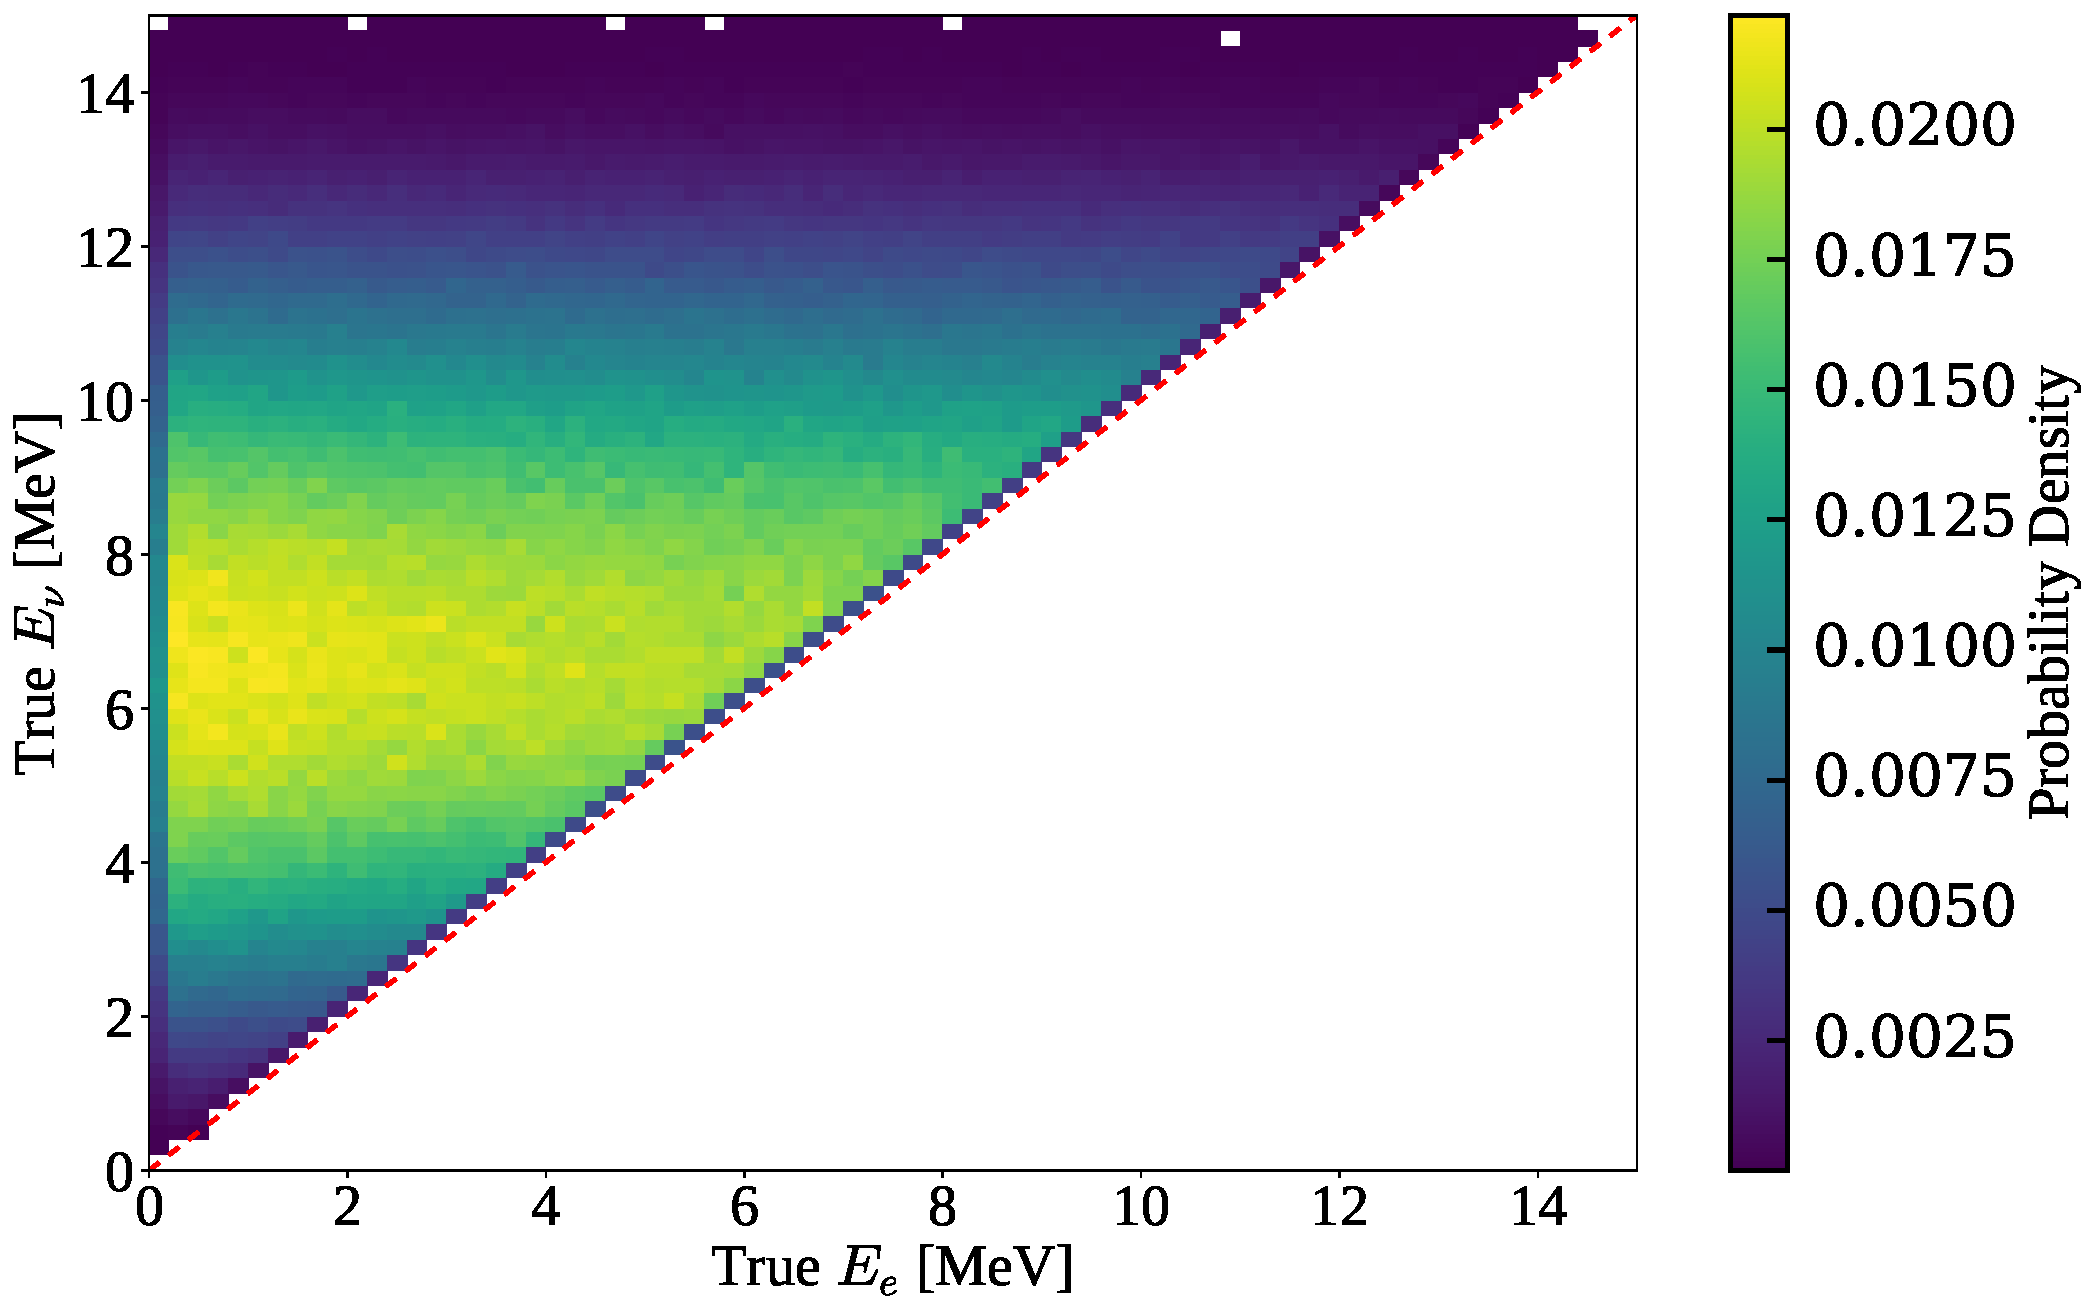
\includegraphics[width=0.8\textwidth]{6_SolarAnalysis/images/b8_eelectrue_vs_enutrue.pdf}
    \caption[]{}
    \label{fig:smellie_laserball_water_ext_length_est}
\end{figure}

\subsubsection{Path Lengths and Transmission Coefficients}
Section~\ref{sec:optical_processes} also discusses the measured refractive indices as a function of wavelength for the UPW, acrylic, and LABPPO. For a given detector phase, subrun, and PMT, the Collaboration's \texttt{Light Path Calculator} is able to determine the values of $L_{ij,p}^{\mathrm{inner}}(\lambda_{j})$ as well as the combined Fresnel transmission coefficient $T_{ij,p}(\lambda_{j})$. It is assumed that there is negligible uncertainty in these values.

\subsubsection{Measuring the Number of Photoelectrons}
Critical to this analysis is the determination of the mean npe per event in both `far' and `backscatter' PMTs. These two PMT selections have to be approached slightly differently.

The `far' PMTs were selected by first finding the intersection point on the PSUP with a line that passes through both the fibre emission point and the centre of the AV. The 20 PMTs closest to this point were chosen. For a given analysis between a scintillator phase subrun $j$ and a matching water phase subrun, only PMTs inside this selection which were identified as ``good'' (as defined in Section~\ref{sec:combining_beam_profiles}) in both subruns were used. For a given far PMT being used, direct light was isolated by calculating the time residuals of all hits on the PMT, using the ``$t_{\mathrm{emm}} = t_{\mathrm{med}}$'' approach mentioned in Section~\ref{sec:smellie_triggering_daq}. Then, the number of hits observed in a ``tight'' time residual window of $[-5,+5]\,\si{\ns}$ was measured for the PMT of interest. By converting to occupancy and then using a multi-hit correction as described in Eq.~\ref{eq:multihit_correction}, the total npe per event for that PMT was estimated. The uncertainty in this value was given by the Poisson error of the calculated npe. In order to minimise the statistical uncertainty, all individual far npe measurements for a given subrun were combined into one value of the `far' light npe per event, $\mu_{j,p}^{\mathrm{far}}$.

Backscattered PMTs were selected for each fibre by finding the 50 PMTs closest to the fibre emission point. A \tres{} window of $[-30,-10]\,\si{\ns}$ was used for the isolation of backscattered light in each subrun. Like above, the total hits for each PMT was converted into a total npe with associated Poisson error. A final correction was made to account for noise hits: the measured noise rate of a given PMT was calculated using the PULSEGT triggers, as described in Section~\ref{sec:smellie_software}. After accounting for the width of the time window, the corresponding expected number of noise hits was subtracted off of the total measured npe to give the npe per event from direct light only. The npe from far PMTs were combined into one value of the backscattered light npe per event, $\mu_{j,p}^{\mathrm{back}}$. 

Fig.~\ref{fig:smellie_extlength_PMT_selections} shows the time residual distributions for both PMT selections of a simulation of the PQ407 laser being fired through fibre FS007 during the scintillator phase, with \SI{2.2}{\gpl} PPO loading. The simulation used the optical model described in Section~\ref{sec:optical_processes}. The earliest photon track associated with a given PMT hit was classified by the optical processes it underwent. A hit associated with a photon that travelled unimpeded through the detector is classified as `direct'. For this fibre and wavelength combination, the time residual windows used allow for a signal-to-background ratio of XXX for the far PMTs, and XXX for the backscattered PMTs. % FILL IN.

\begin{figure}
    \centering
    \begin{subfigure}{0.98\textwidth}
        \centering
        % 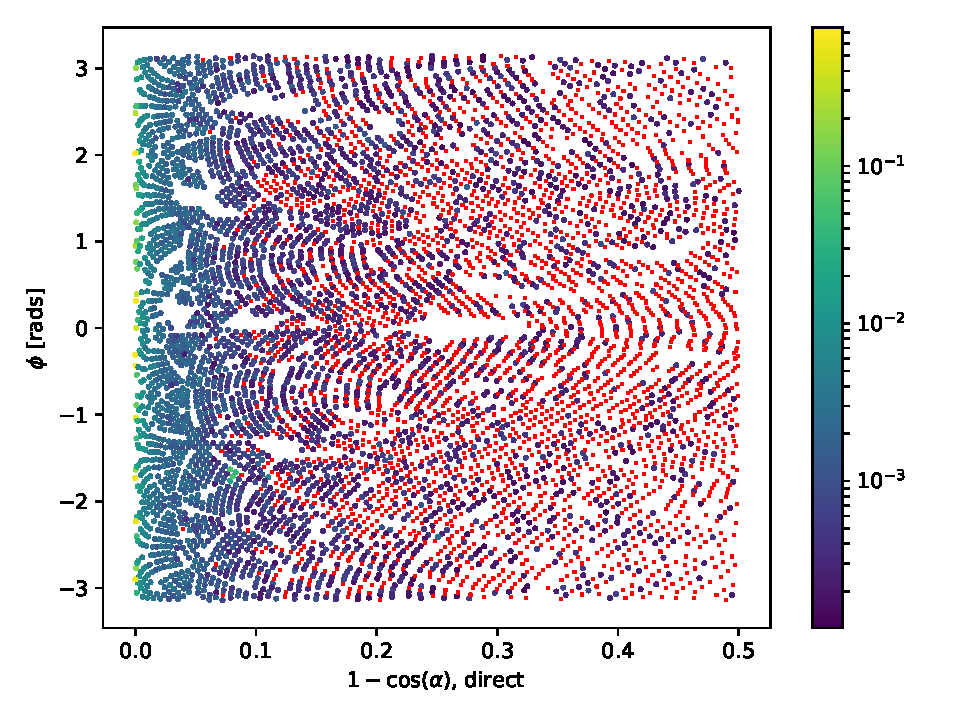
\includegraphics[width=0.74\textwidth]{4_SMELLIESimulation/images/flat_plot_r_FS055_beam_profile_original_6-18-13.pdf}
        \caption{}
        \label{fig:smellie_far_PMT_selection}
    \end{subfigure}
    \begin{subfigure}{0.98\textwidth}
        \centering
        % 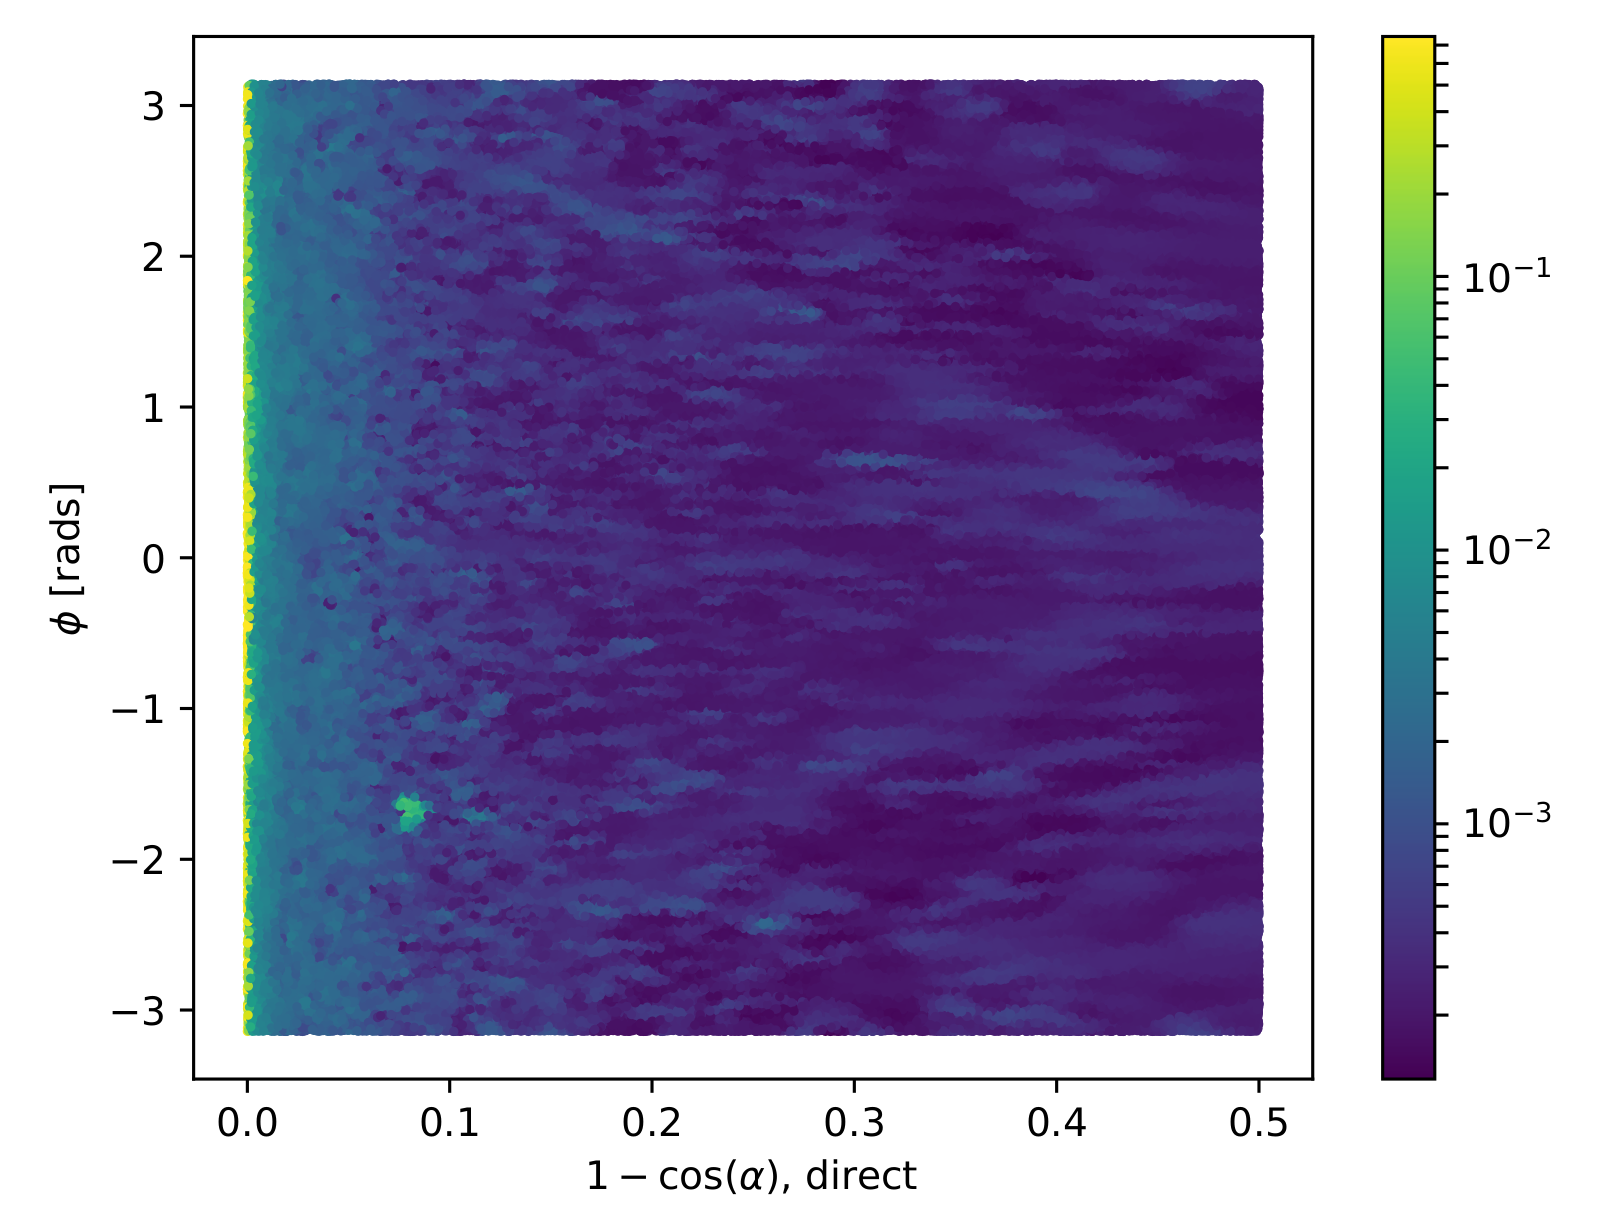
\includegraphics[width=0.74\textwidth]{4_SMELLIESimulation/images/polar_plot_FS055_MC_sampling_old_beam_profile.png}
        \caption{}
        \label{fig:smellie_backscat_PMT_selection}
    \end{subfigure}
    \caption[]{}
    \label{fig:smellie_extlength_PMT_selections}
\end{figure}

$t_{\mathrm{med}}$ was used in this analysis instead of $t_{2}$ because it was found to be far more robust to changes in emission intensity. Fig.~\ref{fig:t2_temm_comparison} shows a comparison of the \tres{} distribution for backscattered PMTs between using $t_{2}$ and $t_{\mathrm{med}}$, at different emission intensities. As can be seen, the $t_{2}$ distribution is biased towards positive \tres{} values, with a bias that is emission-intensity dependent. This is not the case when using $t_{\mathrm{med}}$. 

\begin{figure}
    \centering
    % 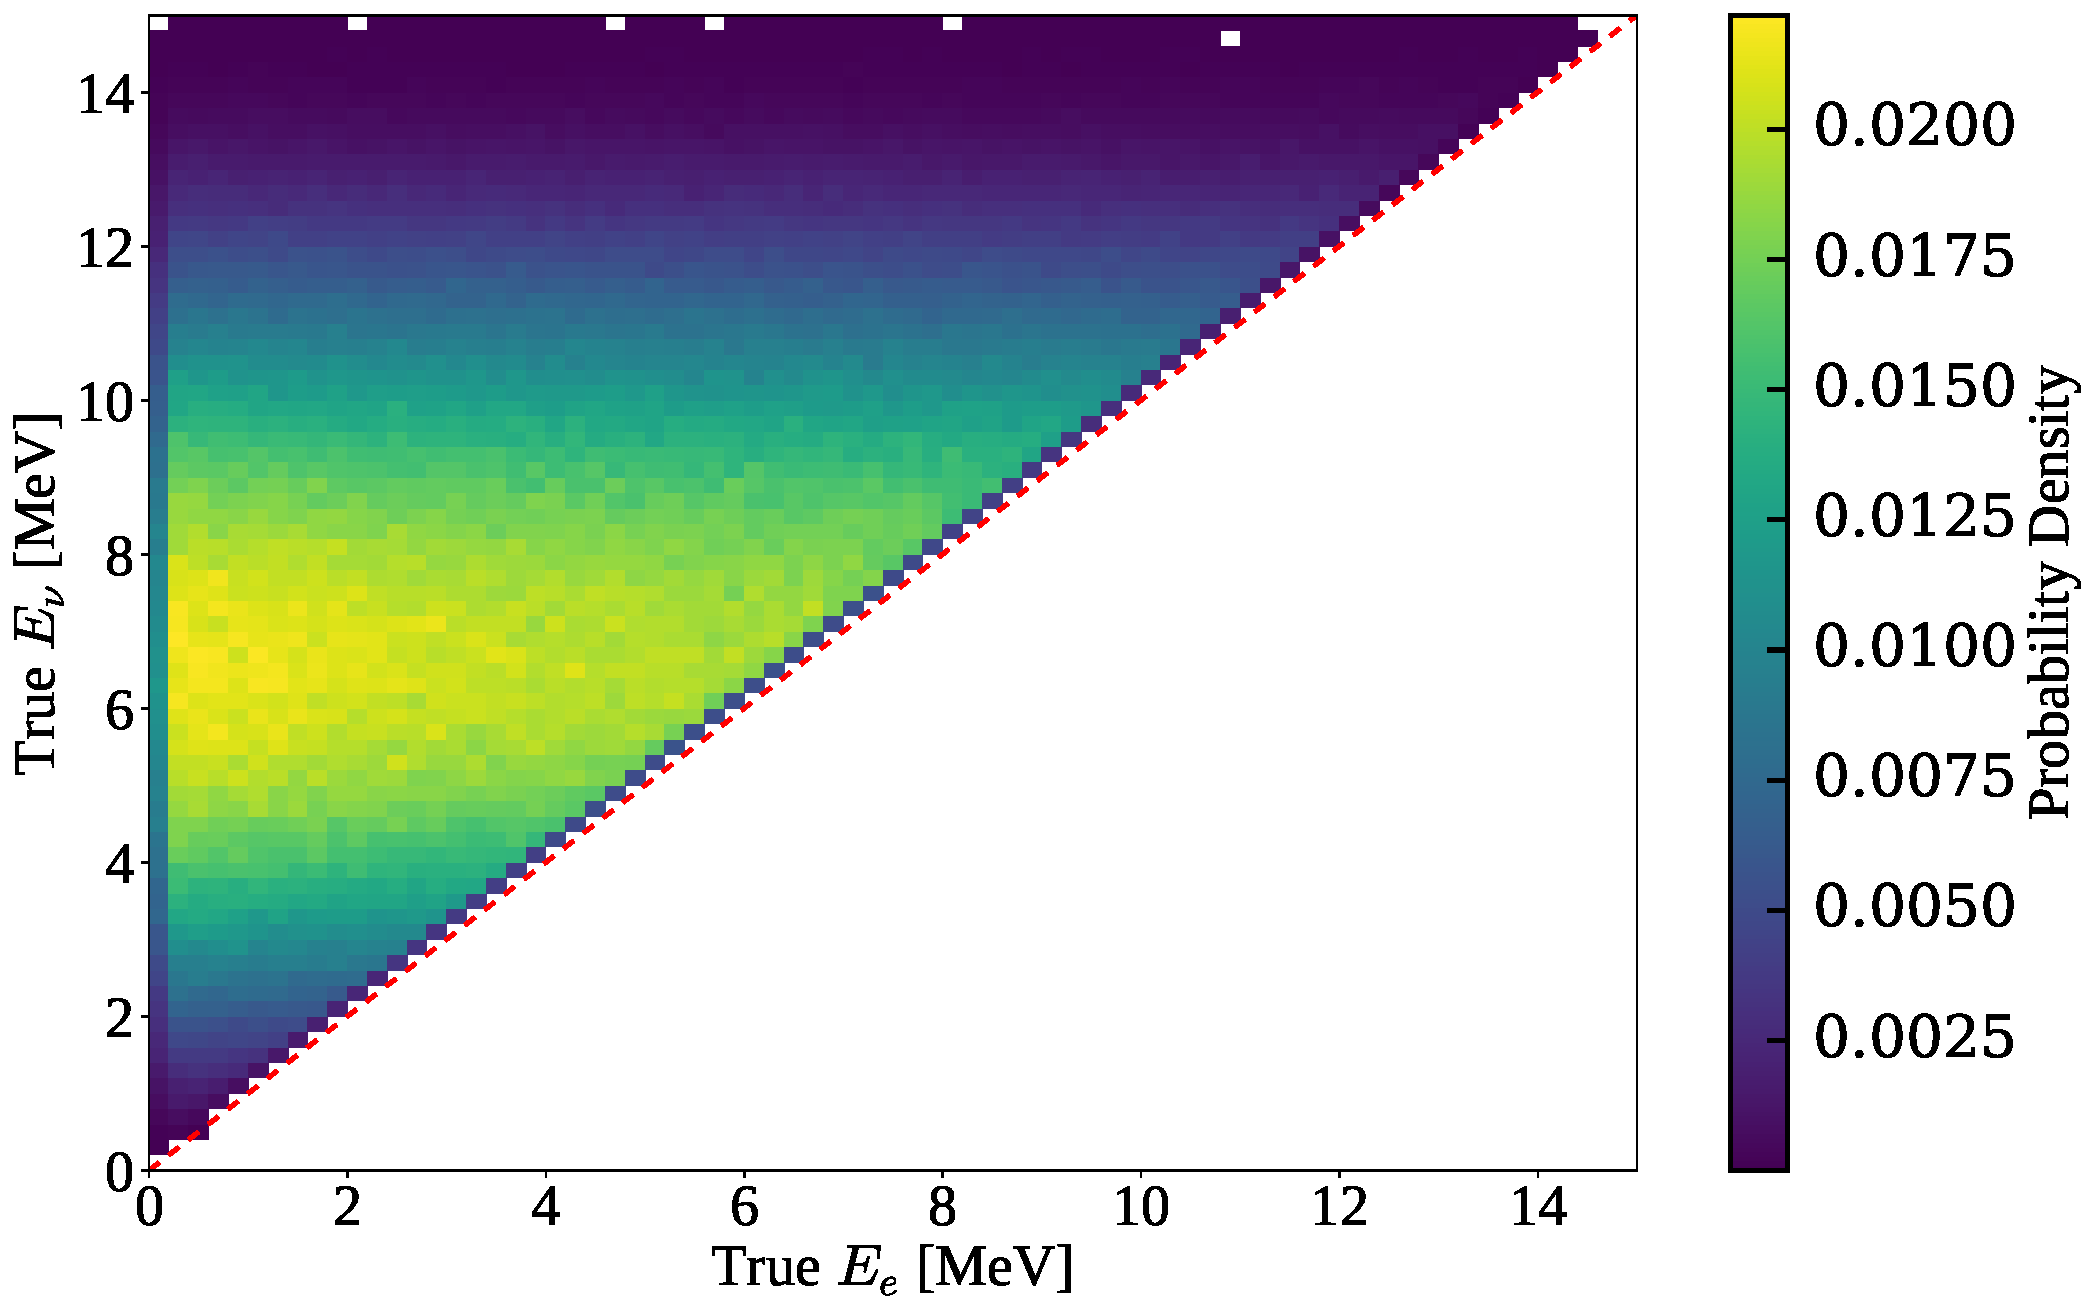
\includegraphics[width=0.8\textwidth]{6_SolarAnalysis/images/b8_eelectrue_vs_enutrue.pdf}
    \caption[]{}
    \label{fig:t2_temm_comparison}
\end{figure}

% \begin{itemize}
%     \item Outline theoretical approach for how one could measure the extinction length of scintillator through a comparison of SMELLIE data between the scintillator and water phases, in the simplified 1 dimensional case with only 2 PMTs.
% \end{itemize}
% [3 pages]

% \subsubsection{Differential Beamspot Refraction}\label{sec:smellie_ext_corrections}
% The correction factor $s_{ij,p}(\lambda_{j})$ is very important for comparing water and scintillator phase data like-for-like. As the SMELLIE beam travels through the AV, refraction bends it by a small amount. However, the amount of this bending will change as a function of the refractive index of the inner detector medium. Because the beam profile drops roughly exponentially as a function of $\alpha$, even small movements in the SMELLIE beam can have a substantial impact on the measured npe for a given beamspot PMT.

% To quantify this effect, SMELLIE events were simulated under ideal conditions in the water phase for every fibre, with the PQ495 laser. Then, the npe per event in the prompt time window was calculated using the same approach described in the previous section. % CONFIRM!!
% The use of the water phase and \SI{495}{\nm} wavelength was chosen so that the impact from optical scattering or absorption would be small. Then, the refractive index of the inner water was modified to match that of LAB, and the above simulations and npe calculations were repeated. The results of this are shown for fibre FS107 in the first two plots of Fig.~\ref{fig:smellie_ref_index_ratio_beamspot}. As can be seen, there is a clear movement of the beam by a polar angle of $\sim\ang{5}$. % CONFIRM!!!
% The movement of other common features in the beamspot, such as the rope shadows and ring structures, can also be seen. There is also a dramatic band of low-npe PMTs that appears only in the latter simulation. This phenomenon will be explained and taken advantage of in Section~\ref{sec:smellie_scatt_new_method} for the scattering analysis.

% \begin{figure}
%     \centering
%     % 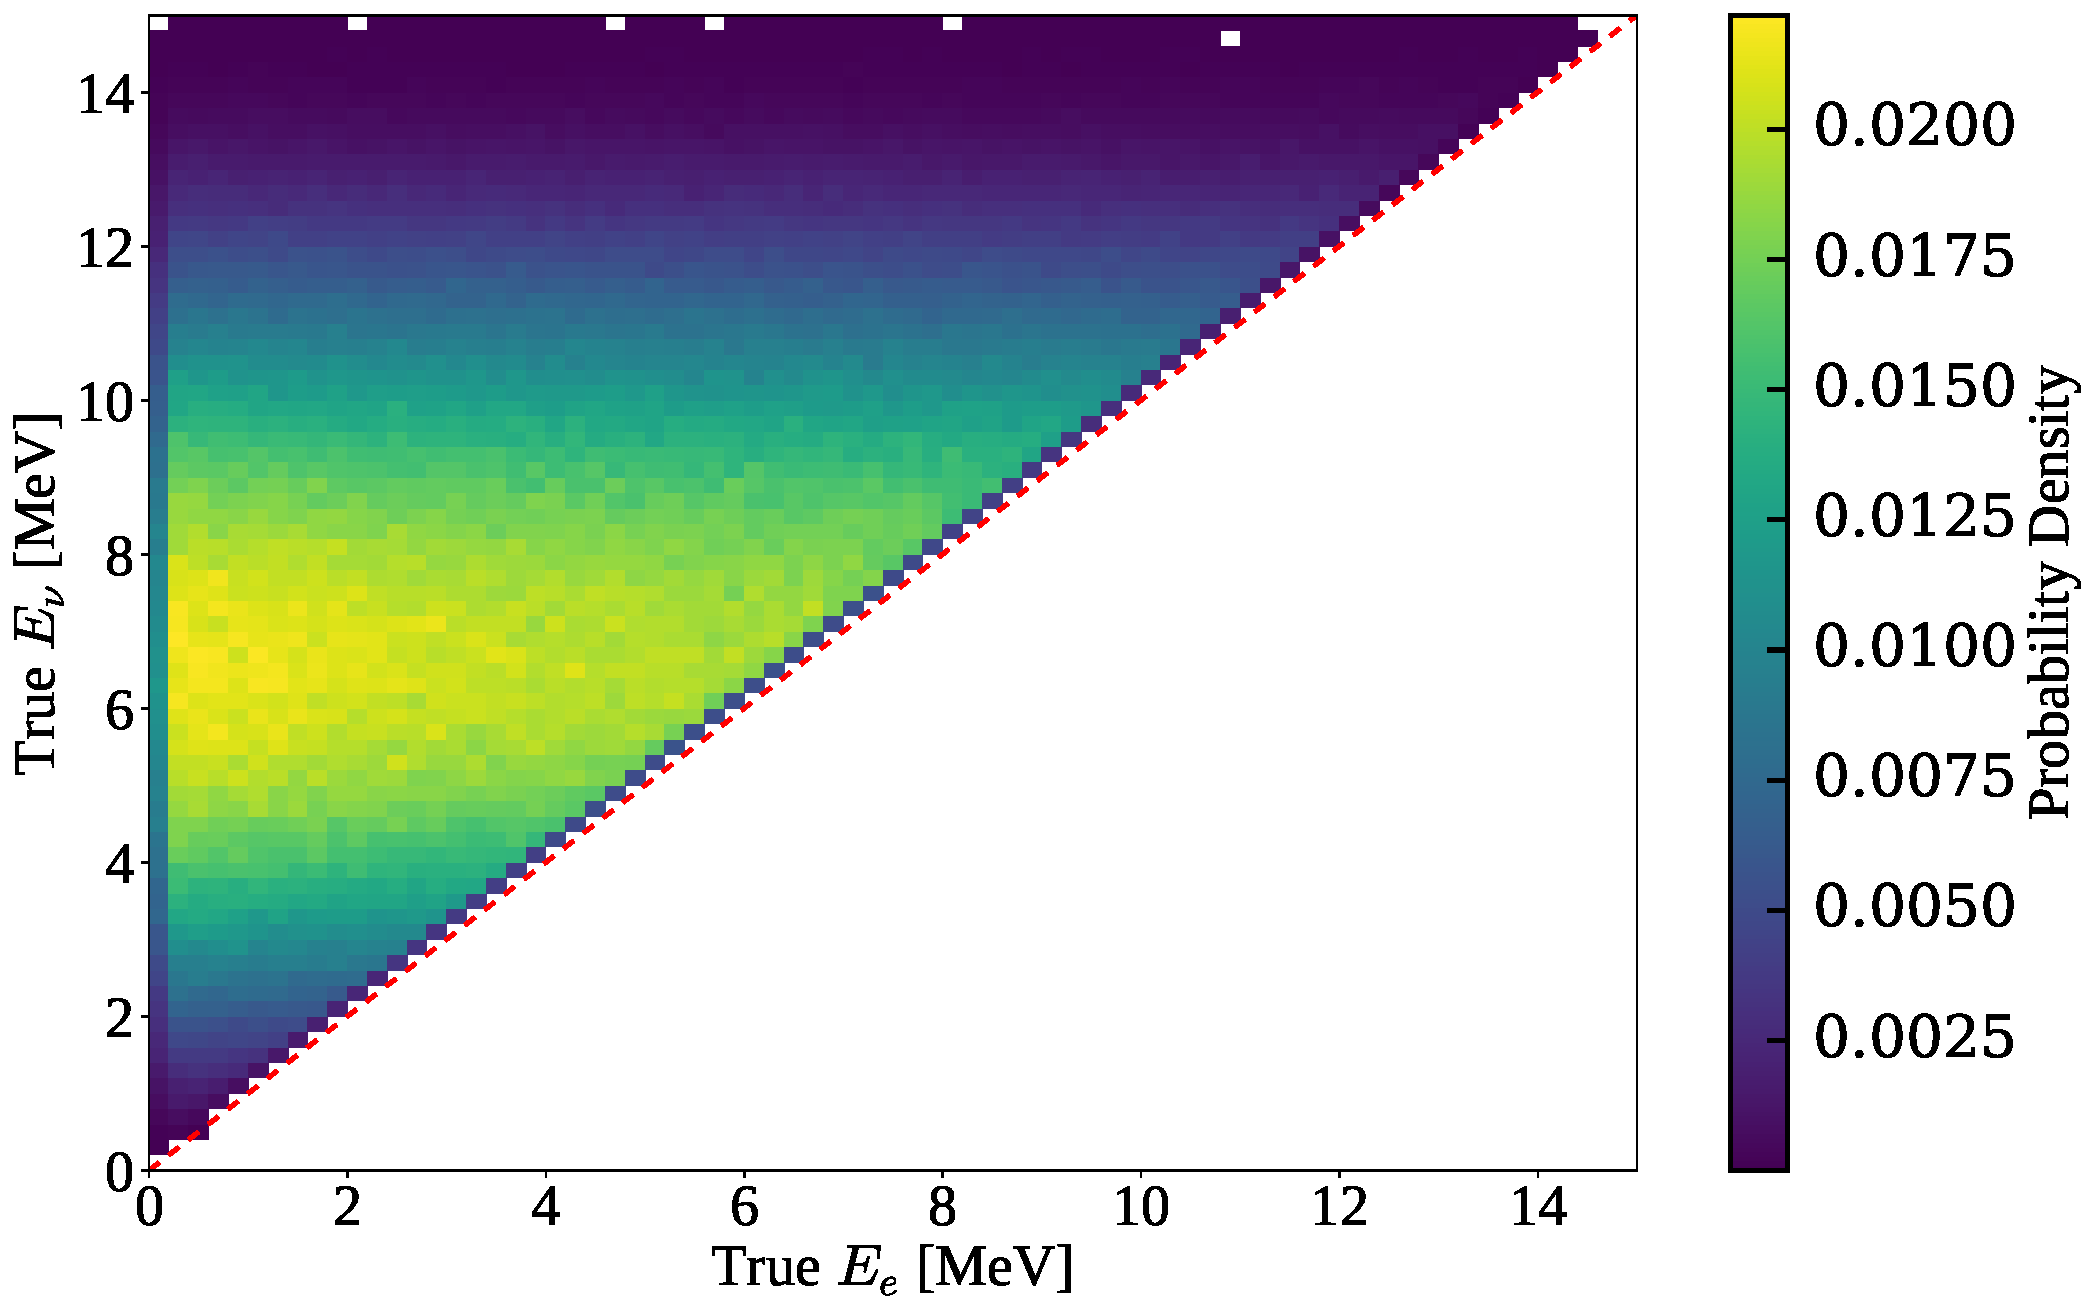
\includegraphics[width=0.8\textwidth]{6_SolarAnalysis/images/b8_eelectrue_vs_enutrue.pdf}
%     \caption[]{}
%     \label{fig:smellie_ref_index_ratio_beamspot}
% \end{figure}

% These simulations were then used to estimate the values of $s_{ij,p}(\lambda_{j})$ in the beamspot. It was assumed that the beam profiles used in simulation were a reasonable model for the beamspot, and there was no wavelength-dependence in these profiles. Assuming that the fractional changes in path lengths relative to their associated extinction lengths are negligible, by using Eq.~\ref{eq:smellie_ext_length_theory} the above ratio will just be:
% \begin{equation}
%     \frac{\mu_{ij,\ce{H_{2}O}}^{\mathrm{beam}}}{\mu_{ij,\ce{H_{2}O}'}^{\mathrm{beam}}}
%     = \frac{T_{ij,\ce{H_{2}O}}}{T_{ij,\ce{H_{2}O}'}}\cdot
%     \frac{b_{ij,\ce{H_{2}O}}\epsilon_{ij,\ce{H_{2}O}}}{b_{ij,\ce{H_{2}O}'}\epsilon_{ij,\ce{H_{2}O}'}}
%     = \frac{T_{ij,\ce{H_{2}O}}}{T_{ij,\ce{H_{2}O}'}}\cdot s_{ij,\mathrm{scint}},
% \end{equation}
% where $p = \ce{H_{2}O}'$ corresponds to the simulation with the modified refractive index. Therefore, the values of $s_{ij,\mathrm{scint}}$ can be estimated by:
% \begin{equation}
%     s_{ij,\mathrm{scint}} = 
%     \frac{\mu_{ij,\ce{H_{2}O}}^{\mathrm{beam}}}{\mu_{ij,\ce{H_{2}O}'}^{\mathrm{beam}}}
%     \cdot \frac{T_{ij,\ce{H_{2}O}'}}{T_{ij,\ce{H_{2}O}}}.
% \end{equation}

% Both the ratio $\frac{\mu_{ij,\ce{H_{2}O}}^{\mathrm{beam}}}{\mu_{ij,\ce{H_{2}O}'}^{\mathrm{beam}}}$ and the derived value for $s_{ij,\mathrm{scint}}$ for fibre FS107 are shown in Fig.~\ref{fig:smellie_ref_index_ratio_beamspot}. % ADD SOME COMMENTS HERE?? ALSO ABOUT ASSUMPTION OF BEAM PROFILE


% \begin{itemize}
%     \item Not doing analysis with just 2 PMTs, of course! Can combine results from multiple PMTs within a beamspot: I explain how here.
% \end{itemize}
% [2 pages]

% \subsubsection{Corrections Between the Water and Scintillator Phases}
% \begin{itemize}
%     \item Note the complications that we have to deal with. Namely, the differing refractive indices of the media bending the beamspot differently in the phases, as well as the method used to estimate $t_{\textrm{emm}}$.
%     \item Explain how we deal with these, the former through MC simulation.
% \end{itemize}
% [2 pages]


% \subsection{Validation of the Analysis in Simulation}
% \begin{itemize}
%     \item Show results of this approach being used to measure the extinction length in simulation. How well does it do?
% \end{itemize}
% [3 pages]

\subsection{Results in Data}
\subsubsection{Datasets Used}
The datasets used in this analysis are summarised in Table~\ref{tab:smellie_ext_length_data}. The water phase data all came from run \num{114018}; scintillator phase data was taken at five different points during the scintillator phase, two during the loading of PPO and three afterwards. These datasets match those highlighted in Fig.~\ref{fig:smellie_timeline}.

\begin{table}
    \begin{center}
        \begin{tabulary}{\textwidth}{c L L}
            \hline
            Date & Detector Phase & Runs used \\ \hline \hline
            June 2018 & Water Phase & \num{114018} \\ \hline
            May 2021 & Scintillator Phase, \SI{0.6}{\gpl} PPO & \num{270856}, \num{270857}, \num{270858}, \num{270862} \\
            October 2021 & Scintillator Phase, \SI{1.1}{\gpl} PPO & \num{275674}; \num{275676}; \num{275678}; \num{275680} \\
            May 2022 & Scintillator Phase, \SI{2.2}{\gpl} PPO & \num{300706}; \num{300708}; \num{300710}; \num{300712}; \num{300715}; \num{300748} \\
            July 2022 & Scintillator Phase, \SI{2.2}{\gpl} PPO & \num{302628}; \num{302630}; \num{302632}; \num{302634}; \num{302636} \\
            June 2023 & Scintillator Phase, \SI{2.2}{\gpl} PPO & \num{310292}; \num{310294}; \num{310296}; \num{310298}; \num{310303} \\\hline
        \end{tabulary}
    \end{center}
    \caption[Datasets used in this analysis]
    {Datasets used in this analysis.}
    \label{tab:smellie_ext_length_data}
\end{table}

`Medium' intensity subruns from the PQ407 laser were used in this study. % CONFIRM - MIGHT CHANGE!!
Fibres FS193 and FS293 were not used as they failed to ever allow a substantial amount of light through them; FS207 was also not used as there was no beam profile distribution made for that fibre. Every scintillator phase subrun being used was matched to an equivalent water phase subrun.

The sensitivity of the extinction length measurement is strongly dependent on the ratio of that extinction length to the length scale of the AV. Very long extinction lengths are difficult to measure because only a small amount of light is expected to be lost due to scattering or absorption. In contrast, at short extinction lengths only a very small amount of light will reach the other side without being extinguished; the dominant source of hits will come from scattered or re-emitted light.

As an example, Fig.~\ref{fig:smellie_PQ375_far_pmts_components} shows the expected optical component breakdown for hits from far PMTs from fibre FS007 due to laser PQ375, using the current \texttt{RAT} model of the \SI{2.2}{\gpl} LABPPO scintillator phase detector. Because the short extinction length at this wavelength relative to the diameter of the AV, typically there would only be one hit in the beamspot region per event. This meant that $t_{\mathrm{med}}$ would correspond to that hit's time, and because there is an overlap between the beamspot and far PMTs for this fibre, a large spike at $\tres{} = 0$ can be observed. Importantly, the amount of direct light seen in the far PMTs in this simulation is entirely sub-dominant to the re-emitted light. Without accounting for this re-emitted light, this analysis would over-estimate the extinction length substantially. In contrast, it has already been shown in Fig.~\ref{fig:smellie_far_PMT_selection} that the contribution of re-emitted light to the PQ407 laser is expected to be sub-dominant.

\begin{figure}
    \centering
    % 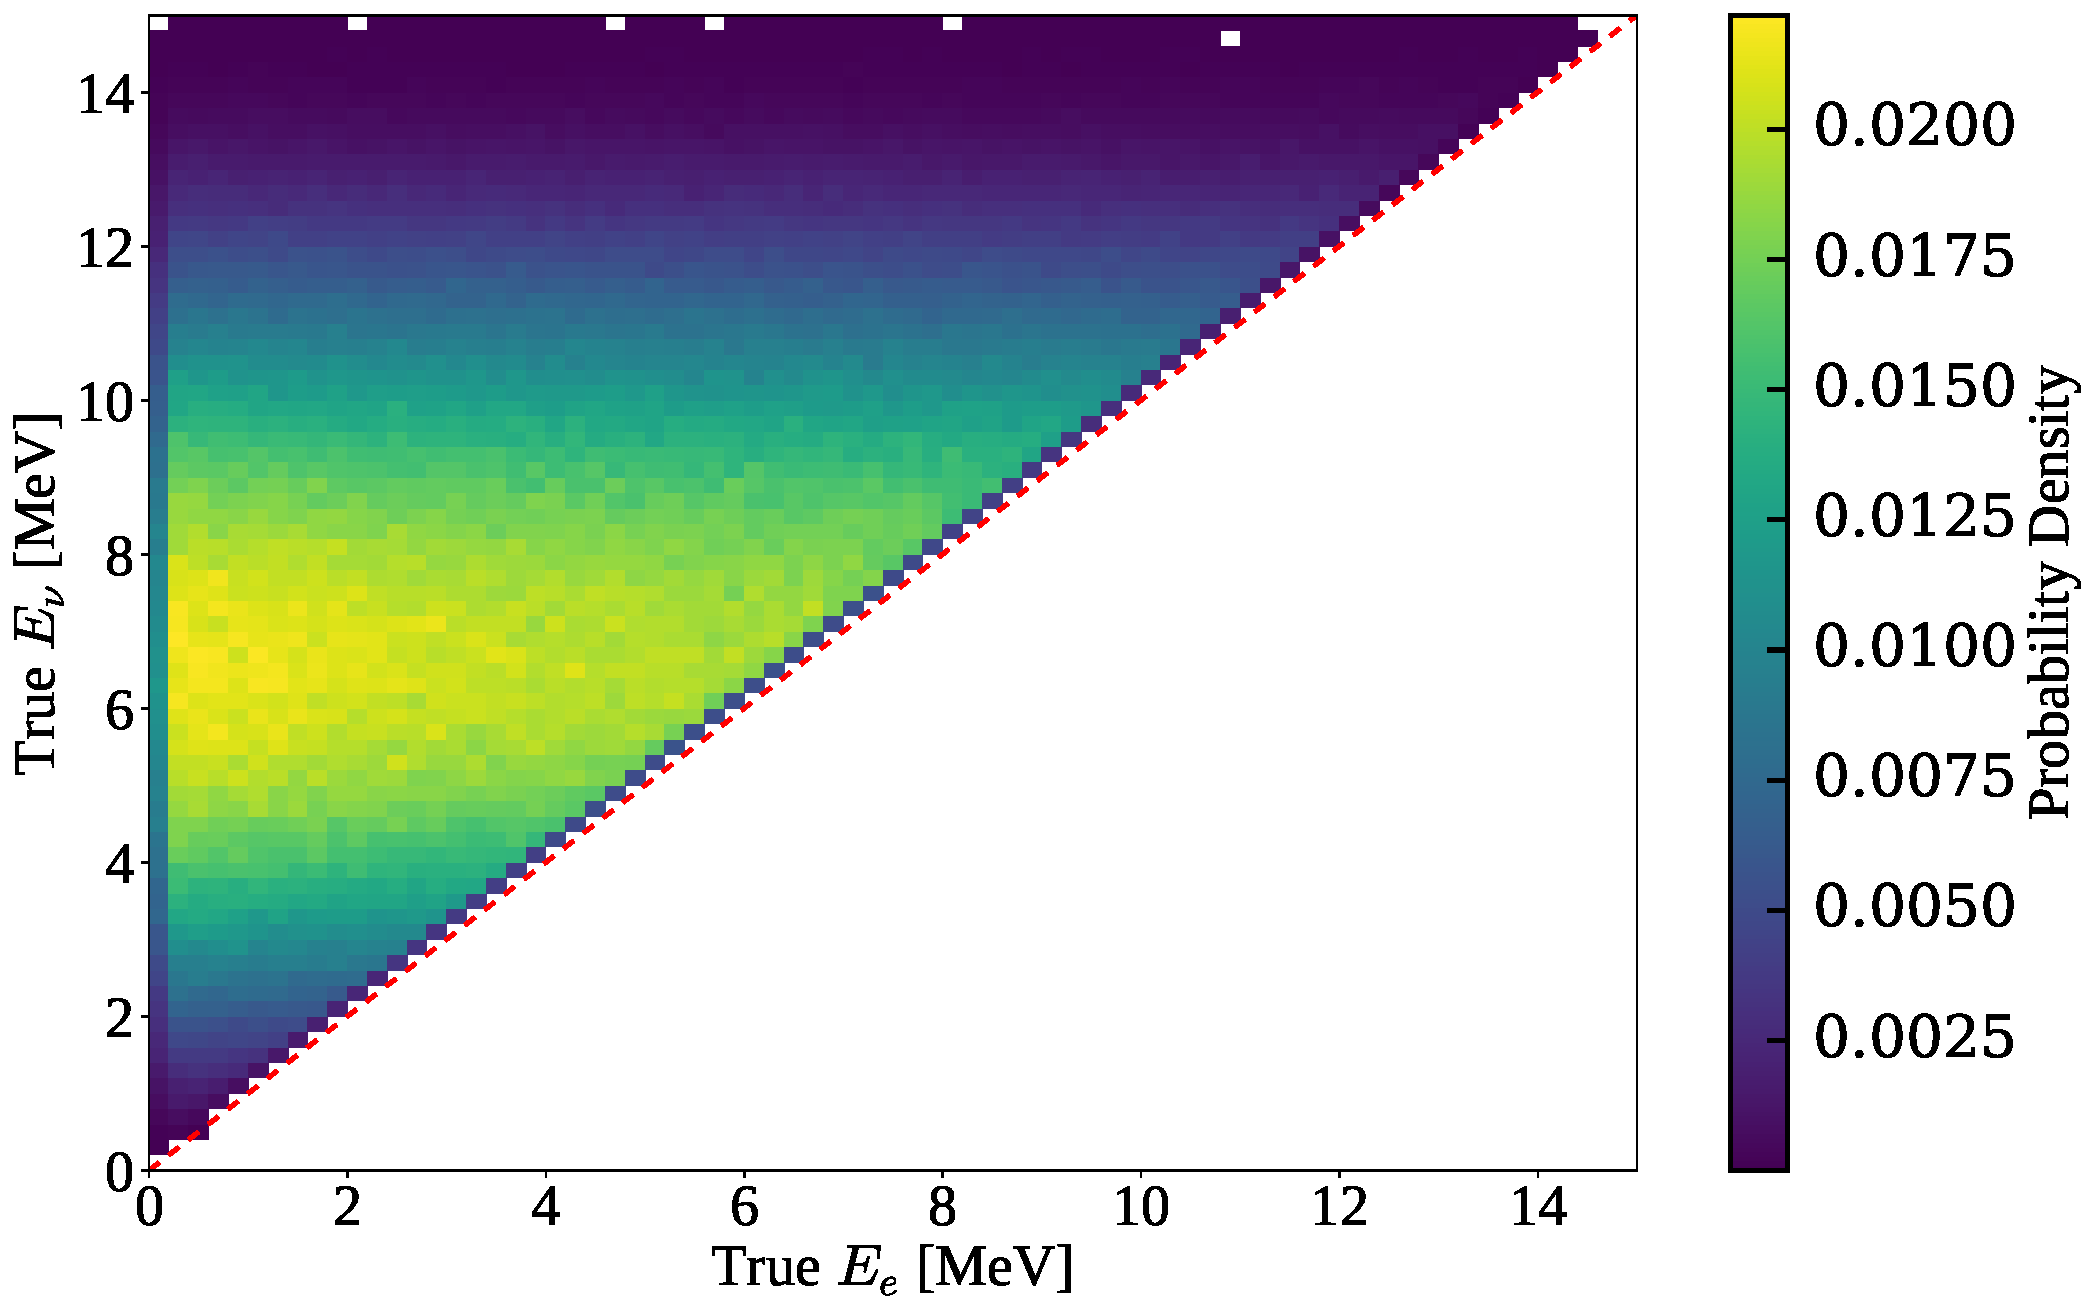
\includegraphics[width=0.8\textwidth]{6_SolarAnalysis/images/b8_eelectrue_vs_enutrue.pdf}
    \caption[]{}
    \label{fig:smellie_PQ375_far_pmts_components}
\end{figure}

For the PQ407 laser, an important background can be scattered light. This becomes most relevant for the \ang{10} and \ang{20} fibres, as the direction of the far PMTs are somewhat distant from the beamspot, so the intensity of direct light is substantially less than that of the ang{0} fibres. A simulation of this is shown in Fig.~\ref{fig:smellie_PQ407_FS107_far_pmts_components} for fibre FS107 in the \SI{2.2}{\gpl} scintillator phase. The proportion of direct light signal to background components in the $[-5,+5]\,\si{\ns}$ window is substantial. As a result, any measurement of $R_{s}$ would be systematically off. % have to introduce R_s, R_w notation earlier.
With similar simulations for all other fibres, it was found that all \ang{0} fibres achieved a signal-to-background ratio of over 95\%. No other fibres were able to achieve a signal purity close to this value. Because of this, only \ang{0} fibres were used for actual extinction length calculations in this analysis. Data from the other fibres was still processed, but only used for comparison, as will be seen in the next section.

\begin{figure}
    \centering
    % 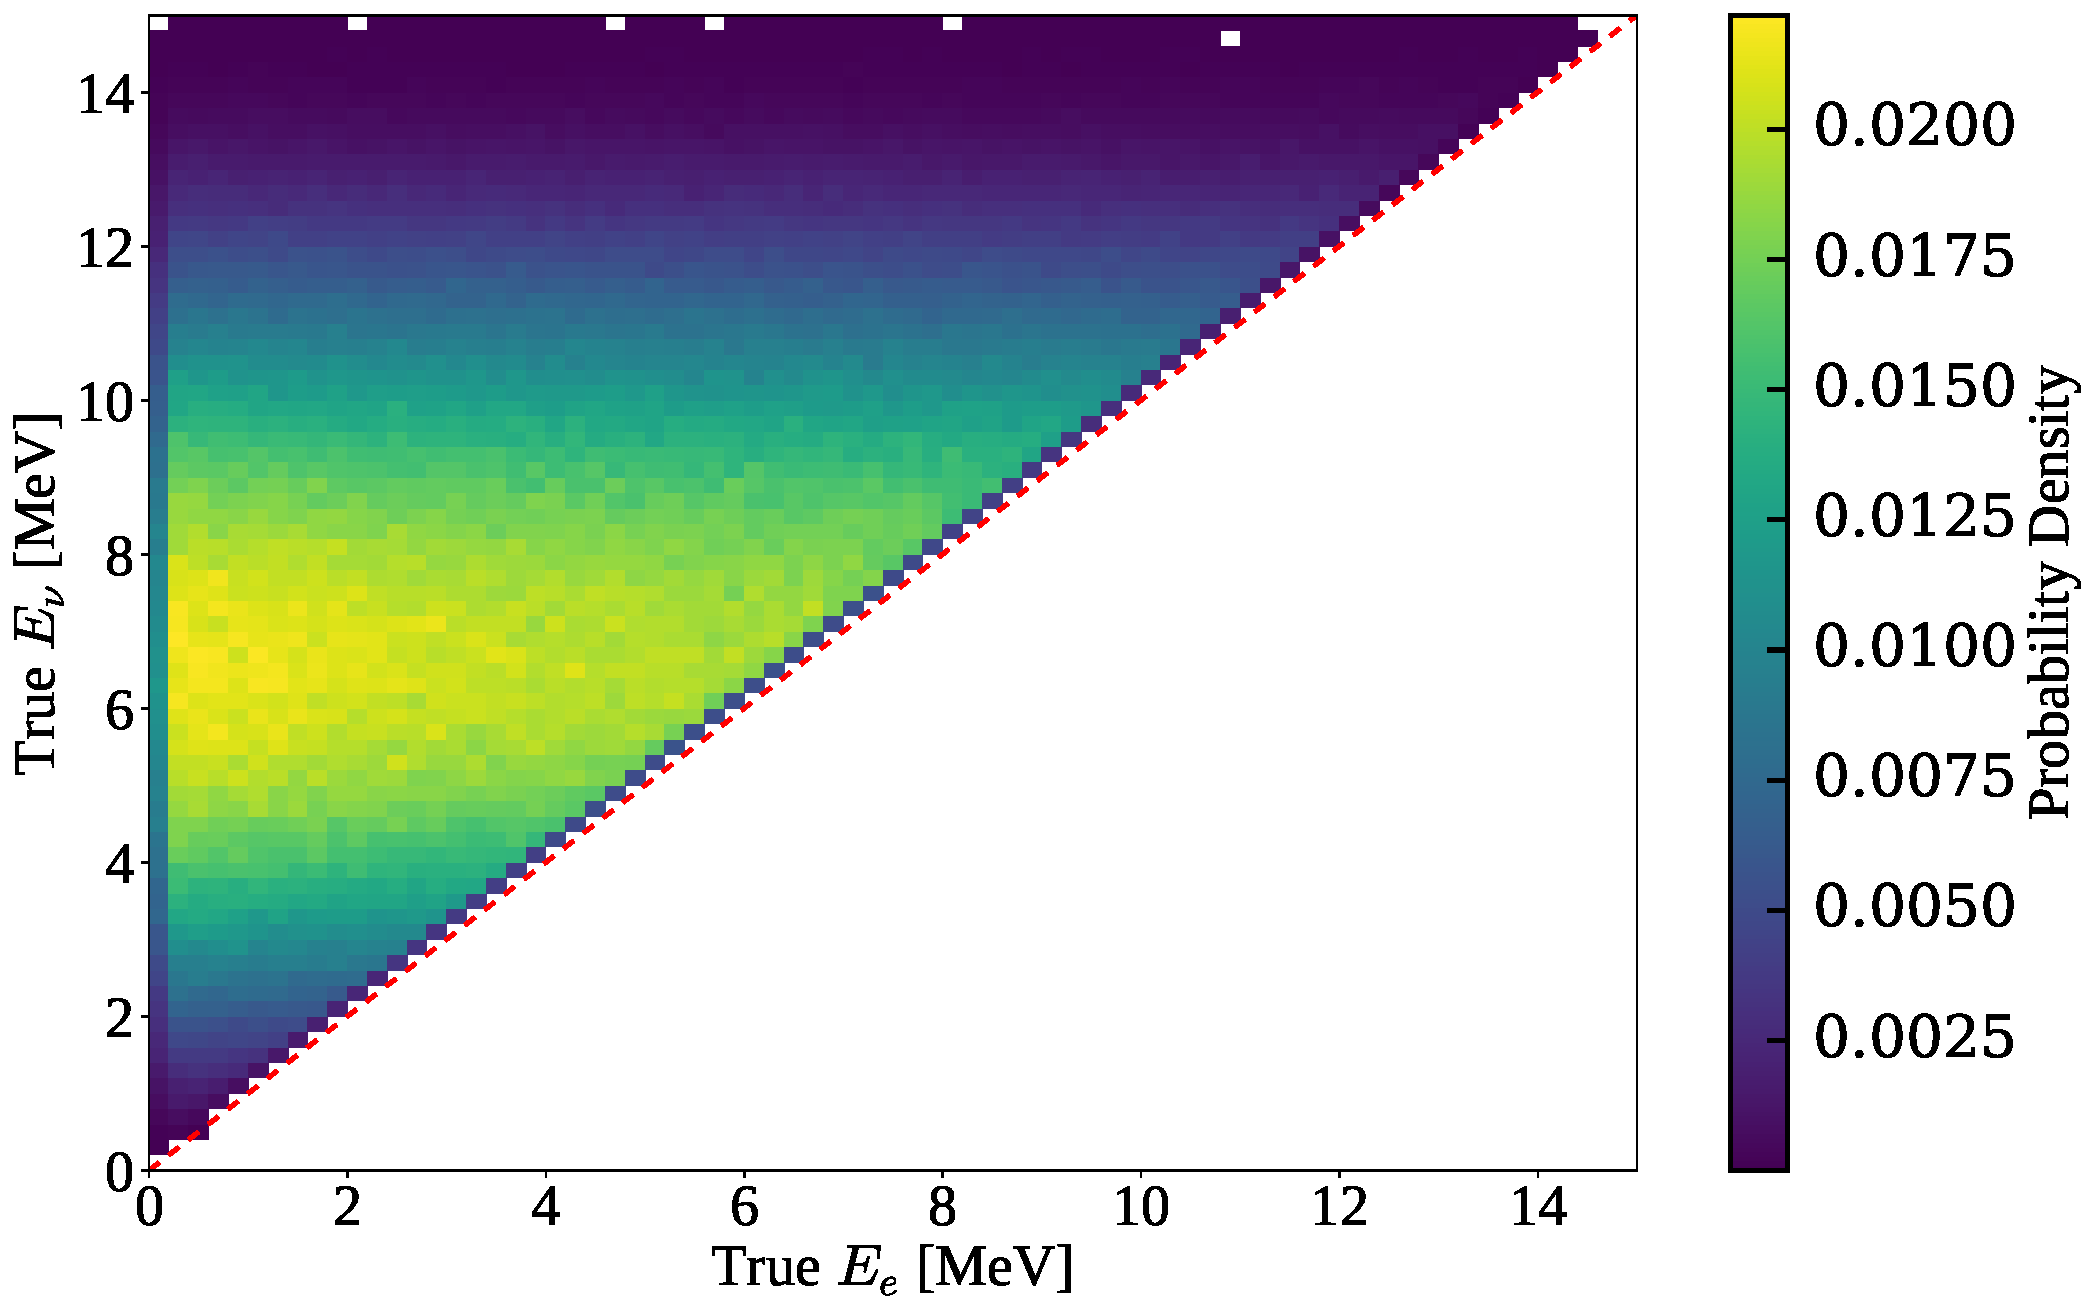
\includegraphics[width=0.8\textwidth]{6_SolarAnalysis/images/b8_eelectrue_vs_enutrue.pdf}
    \caption[]{}
    \label{fig:smellie_PQ407_FS107_far_pmts_components}
\end{figure}

\subsubsection{Results and Discussion}

\begin{sidewaysfigure}
    \centering
    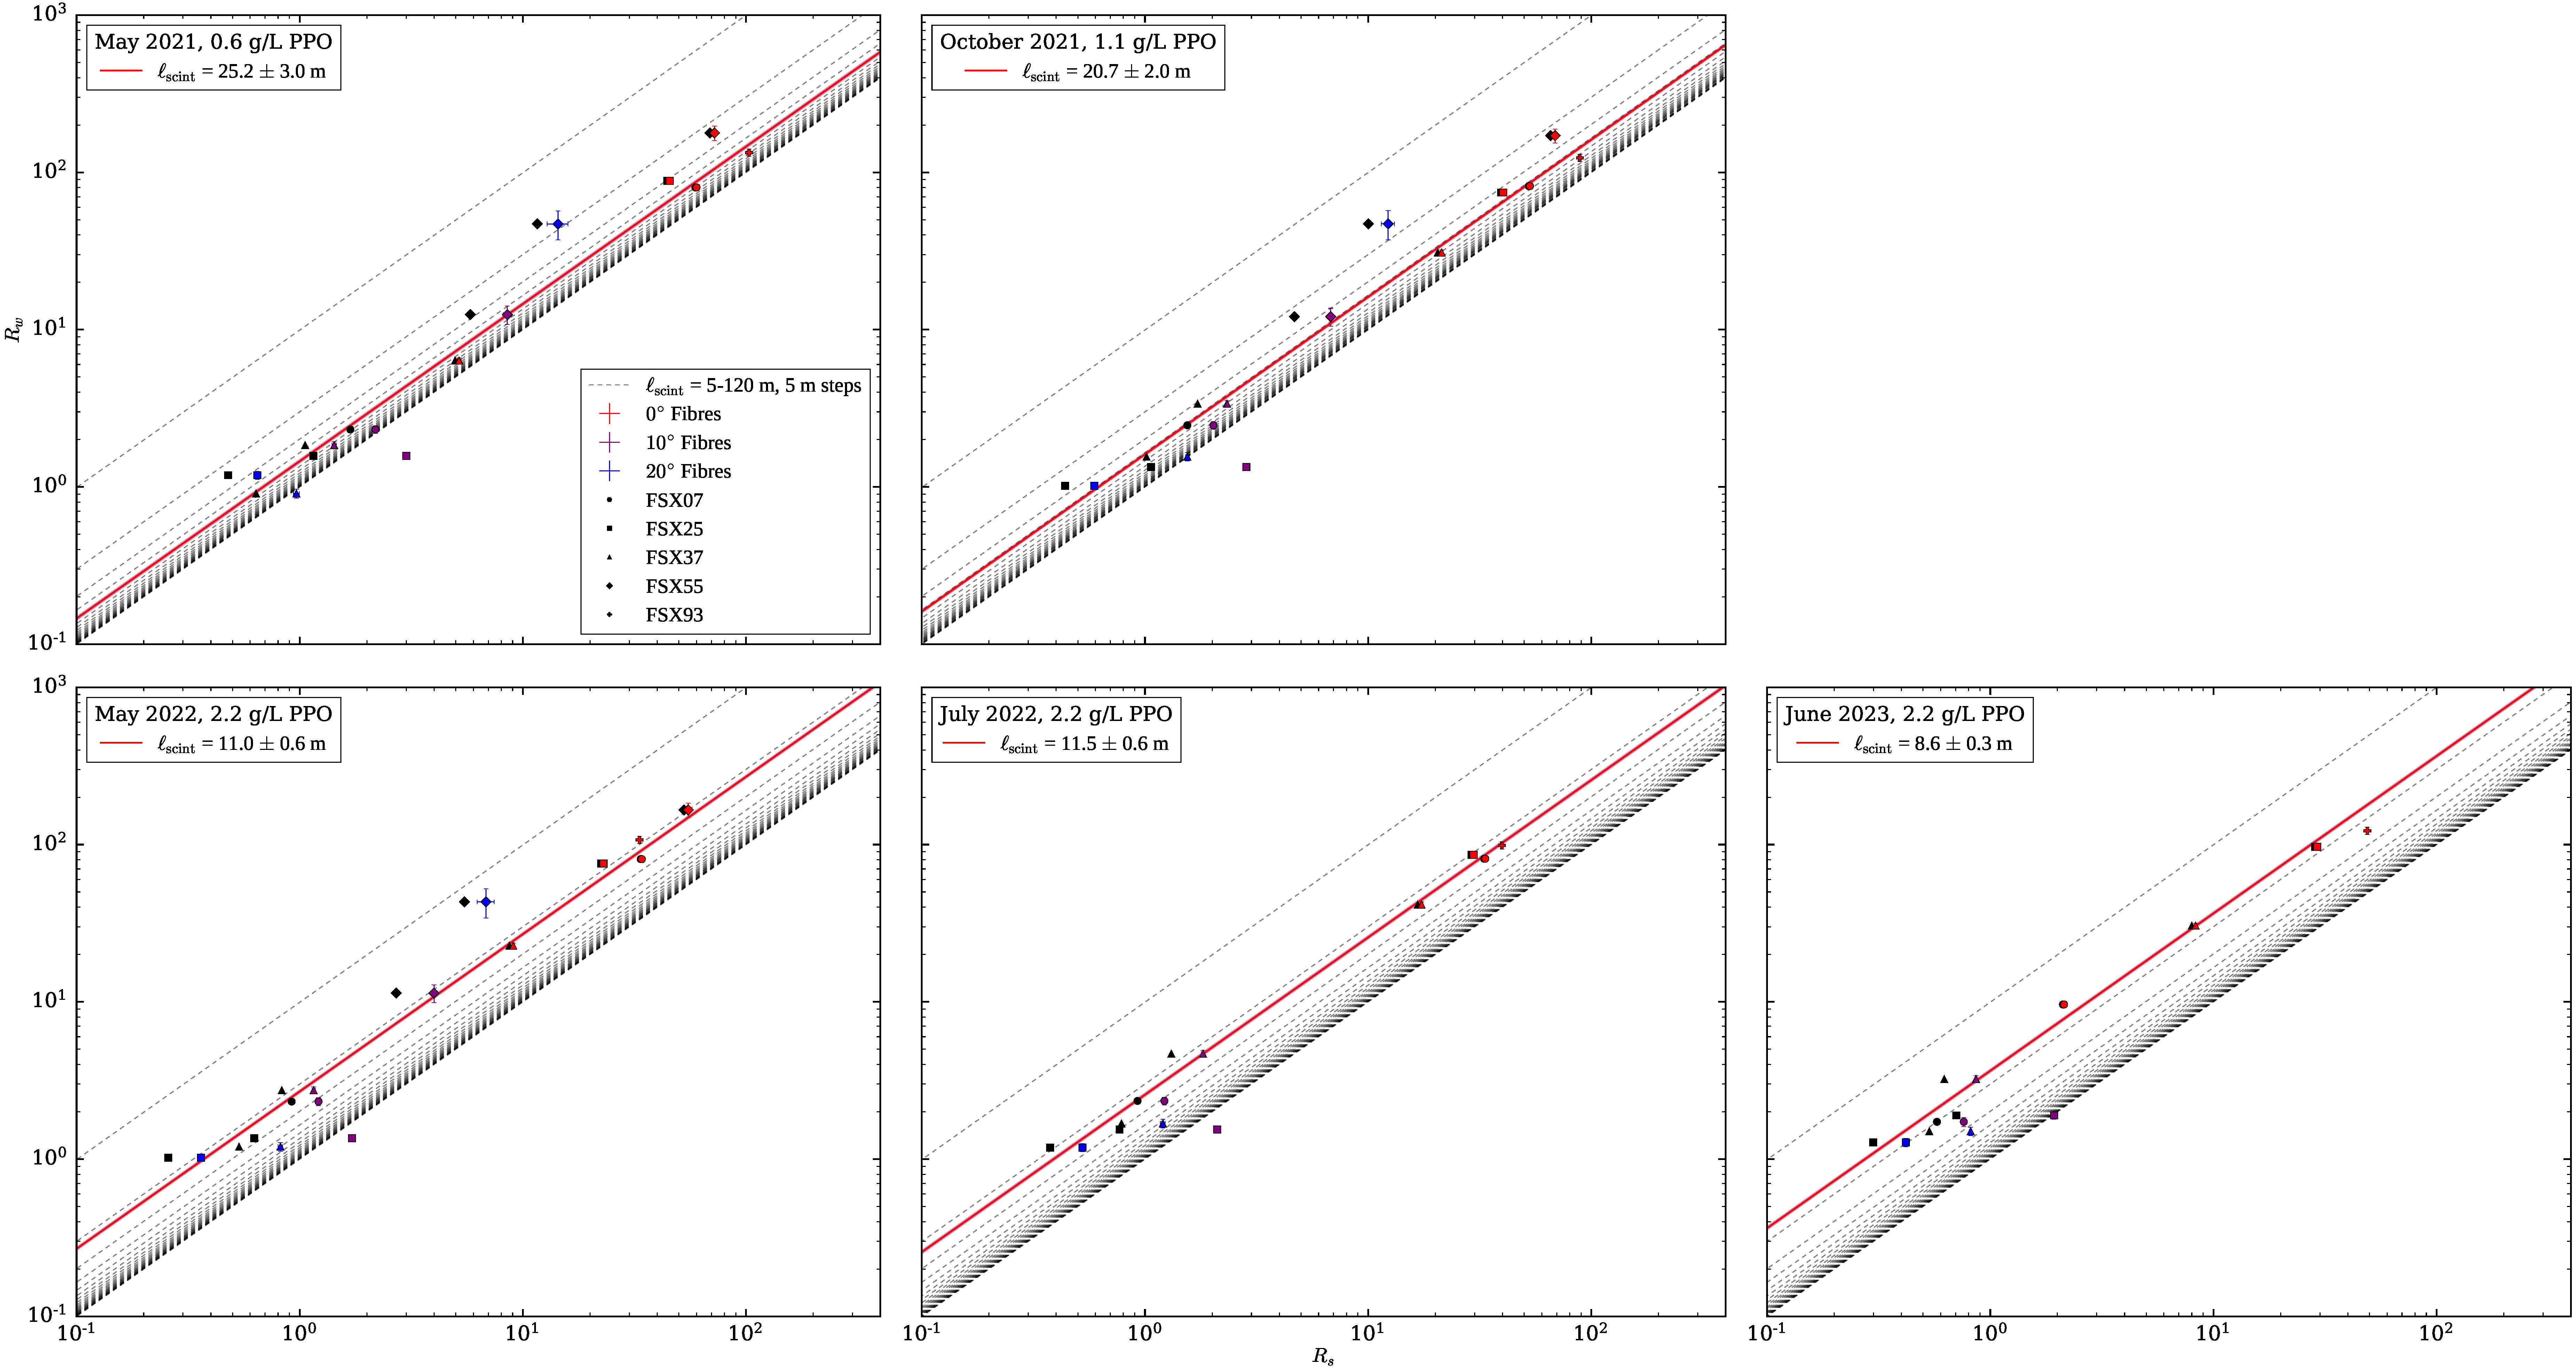
\includegraphics[width=\textwidth]{5_SMELLIEAnalysis/images/rsrw_plot_combined_PQ405.pdf}
    \caption[Results of the extinction length analysis using the PQ407 laser]
    {Results of the extinction length analysis using the PQ407 laser.}
\end{sidewaysfigure}



% \begin{itemize}
%     \item Describe the data used in this analysis, both water and scintillator, which can be shown in a table.
%     \item Show examples of analysis of data in action for \SI{375}{\nm} data: typical $t_{\textrm{res}}$ distributions of backscattered and beamspot PMTs; calculation of that particular extinction length measurement, followed by the graph for extinction length in \SI{375}{\nm} over all fibres and time periods.
%     \item Discuss what results can be seen in this plot: consistency between fibres, the expected change as a function of PPO concentration, and stability of the extinction length during the main \SI{2.2}{\gpl} scintillator phase.
%     \item Compare results to those made by Ben ex-situ: are they in agreement? If not, what possible systematics could there be? The main one for my analysis is likely to be uncertainties in the simulated beam profile that leak through into the refractive index correction of the beamspot. For the ex-situ analysis, the value of the extinction length obtained is achieved through background subtraction at some long wavelength, and the particular choice of this wavelength can lead to systematic changes in the obtained extinction length.
%     \item Look at results at longer wavelengths: can anything reasonably be said at these longer wavelengths? Why/why not?
%     \item Finally: describe any conclusions that can be reached, in particular whether we can affirm the optics model we use in RAT.
% \end{itemize}
% [8 pages]

{
\color{blue}
\section{Scattering Analysis}\label{sec:scattering_analysis}
\subsection{Historical Approaches and the Problem of Systematics}
\begin{itemize}
    \item Comparison to MC is necessary in scattering analysis, compared to merely being needed as a correction factor. This is because of the angular dependence of scattering. As a result, we can be far more susceptible to systematics from poor modelling!
    \item As a warning, show how Krish's/Esther's approach to the SMELLIE scattering analysis suffers majorly from these systematic effects. Requires describing their analysis approach briefly, and then explaining how the systematics described in Section~\ref{sec:smellie_systematics} lead to major problems with this approach.
    \item Motivates the need for either reduced systematics, or an alternative analysis approach that is more robust to them!
\end{itemize}
[2 pages]
\subsection{New Methodology}\label{sec:smellie_scatt_new_method}
\subsubsection{Signal Region Selection}
\begin{itemize}
    \item Propose the new analysis approach: looking at light in the ``bad light-path'' PMT region. Define what this region is.
    \item Give qualitative argument for why we expect this region to be robust to the beam profile systematics: dominated by the scattered signal as no direct light can make it here, and changes to beam profile should get ``smeared out'' after scattering.
    \item Show how simulations indicate this should be a region with a very high purity of scattered light, and (assuming all else being equal) robust to beam profile uncertainties.
    \item Confirm robustness of selected PMT region to uncertainties in AV offset and fibre position.
\end{itemize}
[5 pages]
\subsubsection{Measuring the Emission Intensity}\label{sec:smellie_intensity}
\begin{itemize}
    \item Remaining systematics is now in the calculation of an average absolute emission intensity.
    \item Show how various methods don't work particularly well: whole detector npe, beamspot npe, backscattered light npe, ``bad light-path'' PMTs but at later times. Explain why it goes wrong for each method.
    \item Look at "beamspot but excepting the central bit": if that works well, then we can continue!
    \item Otherwise, we'll have to live with measuring relative scattering lengths instead of absolute amounts, using the outer water back-scattering as a measure of the relative emission intensity.
\end{itemize}
[4 pages]
\subsection{Results}
\begin{itemize}
    \item Actually do the proposed analysis on data, versus time and wavelength. Do the results seem consistent between fibres? Are they sensible values?
\end{itemize}
[5 pages]
[33 PAGES TOTAL]
}